% В этом документе преамбула

\documentclass[a4paper,12pt]{article}

\usepackage{lscape} % горизонтальный режим
\usepackage{pdflscape}

\usepackage{multicol}
\usepackage{algorithm}
\usepackage{algorithmic}
\usepackage{amssymb}
\usepackage{graphicx}
\usepackage{hyperref}
\usepackage{amsthm}
\usepackage{enumitem}
\usepackage{xcolor}


\usepackage{lipsum} % тестовые тексты

%%% Работа с русским языком
\usepackage{cmap}					% поиск в PDF
\usepackage{mathtext} 				% русские буквы в формулах
\usepackage[T2A]{fontenc}			% кодировка
\usepackage[utf8]{inputenc}			% кодировка исходного текста
\usepackage[english,russian]{babel}	% локализация и переносы
\usepackage{indentfirst}			% чтобы первый абзац в разделе отбивался красной строкой
\frenchspacing						% тонкая настройка пробелов
\usepackage{gensymb}				% символы по типу градусов
\usepackage{algorithm}				% для алгоритмов
\usepackage{algorithmic}			% для алгоритмов

%%% Приведение начертания букв и знаков к русской типографской традиции
\renewcommand{\epsilon}{\ensuremath{\varepsilon}}
\renewcommand{\phi}{\ensuremath{\varphi}}			% буквы "эпсилон"
\renewcommand{\kappa}{\ensuremath{\varkappa}}		% буквы "каппа"
\renewcommand{\le}{\ensuremath{\leqslant}}			% знак меньше или равно
\renewcommand{\leq}{\ensuremath{\leqslant}}			% знак меньше или равно
\renewcommand{\ge}{\ensuremath{\geqslant}}			% знак больше или равно
\renewcommand{\geq}{\ensuremath{\geqslant}}			% знак больше или равно
\renewcommand{\emptyset}{\varnothing}				% знак пустого множества

%%% Дополнительная работа с математикой
\usepackage{amsmath,amsfonts,amssymb,amsthm,mathtools,esint} % AMS
\usepackage{wasysym}
\usepackage{icomma} % "Умная" запятая: $0,2$ --- число, $0, 2$ --- перечисление

%% Номера формул
\mathtoolsset{showonlyrefs=true} % Показывать номера только у тех формул, на которые есть \eqref{} в тексте.

%% Перенос знаков в формулах (по Львовскому)
\newcommand*{\hm}[1]{#1\nobreak\discretionary{}
{\hbox{$\mathsurround=0pt #1$}}{}}

%%% Работа с картинками
\usepackage{graphicx}  				% Для вставки рисунков
\graphicspath{{images/}{images2/}}  % папки с картинками
\setlength\fboxsep{3pt} 			% Отступ рамки \fbox{} от рисунка
\setlength\fboxrule{1pt} 			% Толщина линий рамки \fbox{}
\usepackage{wrapfig} 				% Обтекание рисунков текстом

%%% Работа с таблицами
\usepackage{array,tabularx,tabulary,booktabs} 	% Дополнительная работа с таблицами
\usepackage{longtable}  						% Длинные таблицы
\usepackage{multirow}							% Слияние строк в таблице

%----------------------------------------------------------------------------------------------

%%% НАСТРОЙКА СТИЛЕЙ

\newtheoremstyle{break}% name
	{}%         Space above, empty = `usual value'
	{}%         Space below
	{\itshape}% Body font
	{}%         Indent amount (empty = no indent, \parindent = para indent)
	{\bfseries}% Thm head font
	{.}%        Punctuation after thm head
	{\newline}% Space after thm head: \newline = linebreak
	{}%         Thm head spec
\theoremstyle{break}

\newtheorem{lemma}{Лемма}[section]

\newtheoremstyle{mydef}
	{\topsep}%
	{\topsep}%
	{}%
	{}%
	{\bfseries}%
	{}%
	{\newline}%
	{%
		\rule{\textwidth}{0.4pt}\\*%
		\thmname{#1}~\thmnumber{#2}\thmnote{\ -\ #3}.\\*[-1.5ex]%
		\rule{\textwidth}{0.4pt}}%

\theoremstyle{mydef}
\newtheorem{definition}{Определение}[section]

\newtheorem{property}{Свойство}

\newtheoremstyle{inline}%
	{3pt}%
	{3pt}%
	{\normalfont}%
	{}%
	{\bfseries}%
	{}%
	{\newline}%
	{\thmname{#1}\thmnumber{ #2}\thmnote{ (#3)}}%
\theoremstyle{inline}
\newtheorem{exmp}[definition]{Пример}
\newtheorem{theorem}{Теорема}[section]
\newtheorem{axioms}{Аксиомы}[section]
\newtheorem{corollary}{Следствие}[theorem]

\theoremstyle{remark} % "Примечание"
\newtheorem*{nonum}{Решение}
\newtheorem*{remark}{Примечание}

%----------------------------------------------------------------------------------------------

%%% Страница
\usepackage{extsizes} % Возможность сделать 14-й шрифт
\usepackage{geometry} % Простой способ задавать поля
	\geometry{top=15mm}
	\geometry{bottom=35mm}
	\geometry{left=10mm}
	\geometry{right=10mm}

%\usepackage{fancyhdr} % Колонтитулы
% 	\pagestyle{fancy}
 	%\renewcommand{\headrulewidth}{0pt}  % Толщина линейки, отчеркивающей верхний колонтитул
% 	\lfoot{Нижний левый}
% 	\rfoot{Нижний правый}
% 	\rhead{Верхний правый}
% 	\chead{Верхний в центре}
% 	\lhead{Верхний левый}
%	\cfoot{Нижний в центре} % По умолчанию здесь номер страницы

\usepackage{setspace} % Интерлиньяж (межстрочные интервалы)
%\onehalfspacing % Интерлиньяж 1.5
%\doublespacing % Интерлиньяж 2
%\singlespacing % Интерлиньяж 1

\usepackage{lastpage} % Узнать, сколько всего страниц в документе.

\usepackage{soulutf8} % Модификаторы начертания

\usepackage{hyperref}
\usepackage[usenames,dvipsnames,svgnames,table,rgb]{xcolor}
\hypersetup{				% Гиперссылки
    unicode=true,           % русские буквы в раздела PDF
    pdftitle={Заголовок},   % Заголовок
    pdfauthor={Автор},      % Автор
    pdfsubject={Тема},      % Тема
    pdfcreator={Создатель}, % Создатель
    pdfproducer={Производитель}, % Производитель
    pdfkeywords={keyword1} {key2} {key3}, % Ключевые слова
    colorlinks=true,       	% false: ссылки в рамках; true: цветные ссылки
    linkcolor=MidnightBlue, % внутренние ссылки
    citecolor=black,        % на библиографию
    filecolor=magenta,      % на файлы
    urlcolor=blue           % на URL
}

\usepackage{csquotes} % Еще инструменты для ссылок

%\usepackage[style=authoryear,maxcitenames=2,backend=biber,sorting=nty]{biblatex}

\usepackage{multicol} % Несколько колонок

%%% Работа с графикой
\usepackage{tikz}
\usetikzlibrary{calc}
\usepackage{tkz-euclide}
\usetikzlibrary{arrows}
\usepackage{pgfplots}
\usepackage{pgfplotstable}

%%% Настройка подписей к плавающим объектам
% \usepackage{floatrow}	% размещение
\usepackage{caption}	% начертание
\captionsetup[figure]{labelfont=bf,textfont=it,font=footnotesize}	% нумерация и надпись курсивом
% для подфигур: заголовок подписи полужирный, текст заголовка обычный
% выравнивание является неровным (т.е. выровненным по левому краю)
% singlelinecheck = off означает, что настройка выравнивания используется, даже если заголовок имеет длину только одну строку.
% если singlelinecheck = on, то заголовок всегда центрируется, когда заголовок состоит только из одной строки.
\captionsetup[subfigure]{labelfont=bf,textfont=normalfont,singlelinecheck=off,justification=raggedright}

%%% Stuff для листинга
\usepackage{listings}
\usepackage{xcolor}

\usepackage{subcaption}		% размещение рисунков
\usepackage{graphicx}

\colorlet{mygray}{black!30}
\colorlet{mygreen}{green!60!blue}
\colorlet{mymauve}{red!60!blue}

\lstset{
	backgroundcolor=\color{gray!10},  
	basicstyle=\ttfamily,
	columns=fullflexible,
	breakatwhitespace=false,      
	breaklines=true,                
	captionpos=b,                    
	commentstyle=\color{mygreen}, 
	extendedchars=true,              
	frame=single,                   
	keepspaces=true,             
	keywordstyle=\color{blue},      
	language=c++,                 
	numbers=none,                
	numbersep=5pt,                   
	numberstyle=\tiny\color{blue}, 
	rulecolor=\color{mygray},        
	showspaces=false,               
	showtabs=false,                 
	stepnumber=5,                  
	stringstyle=\color{mymauve},    
	tabsize=3,                      
	title=\lstname                
}

% Для извращённых начертаний
\usepackage{mathrsfs}

\usepackage{makecell}
\setcellgapes{3pt}

% Зачёркивание символов
\usepackage{cancel}

% перечисления с буквами
\usepackage{enumitem}

% Римские цифры
\newcommand{\RNumb}[1]{\uppercase\expandafter{\romannumeral #1\relax}}

% Дроби с косой чертой
\usepackage{nicefrac}

% Разделение ячеек таблицы
\usepackage{diagbox}

%----------------------------------------------------------------------------------------------

%% ОБОЗНАЧЕНИЯ ДЛЯ ТВИМС %%

\DeclareMathOperator{\sgn}{\mathop{sgn}}				% ф-ия sgn
\renewcommand{\tg}{\mathop{\mathrm{tg}}\nolimits}		% обозначение тангенса
\DeclareMathOperator{\cov}{\mathop{cov}}				% ковариация
\DeclareMathOperator{\corr}{\mathop{corr}}				% матрица кореляции
\DeclareMathOperator{\var}{\mathop{var}}				% матрица ковариации

\DeclareMathOperator\supp{supp}							% Носитель функции распределения
\DeclareMathOperator{\eq}{\Leftrightarrow}				% Знак эквивалентно

% Борелевская сигма-алгебра
\newcommand{\Borel}{{\mathcal{B}}}
% Мн-во случайных событий
\newcommand{\Event}{{\mathcal F}}

% Кольца чисел N,Z,R,C
\newcommand\NN{{\mathbb N}}
\newcommand\ZZ{{\mathbb Z}}
\newcommand\RR{{\mathbb R}}
\newcommand\CC{{\mathbb C}}

% Спецсимвол "Пусть"
\def\letus{%
	\mathord{\setbox0=\hbox{$\exists$}%
		\hbox{\kern 0.125\wd0%
			\vbox to \ht0{%
				\hrule width 0.75\wd0%
				\vfill%
				\hrule width 0.75\wd0}%
			\vrule height \ht0%
			\kern 0.125\wd0}%
	}%
}
\usepackage{listings}

\lstset{ %
language=Python,                 % выбор языка для подсветки (здесь это С)
basicstyle=\small\sffamily, % размер и начертание шрифта для подсветки кода
numbers=left,               % где поставить нумерацию строк (слева\справа)
numberstyle=\tiny,           % размер шрифта для номеров строк
stepnumber=1,                   % размер шага между двумя номерами строк
numbersep=5pt,                % как далеко отстоят номера строк от подсвечиваемого кода
backgroundcolor=\color{white}, % цвет фона подсветки - используем \usepackage{color}
showspaces=false,            % показывать или нет пробелы специальными отступами
showstringspaces=false,      % показывать или нет пробелы в строках
showtabs=false,             % показывать или нет табуляцию в строках
frame=single,              % рисовать рамку вокруг кода
tabsize=2,                 % размер табуляции по умолчанию равен 2 пробелам
captionpos=t,              % позиция заголовка вверху [t] или внизу [b] 
breaklines=true,           % автоматически переносить строки (да\нет)
breakatwhitespace=false, % переносить строки только если есть пробел
escapeinside={\%*}{*)}   % если нужно добавить комментарии в коде
}

\newcommand{\bolditalic}[1]{\textbf{\textit{#1}}}

\title{Построение и анализ алгоритмов}


\begin{document}
\author{
\href{https://github.com/danilpavlov/latex_lib}{Ссылка} на .tex файлы и все-такое}
\maketitle
\tableofcontents
\newpage

\section{Поиск с возвращением. Метод Монте-Карло}

    \subsection{Идея поиска с возвращением (backtracking)}

    \textit{Поиск с возвращением} (backtracking) является алгоритмическим подходом к решению задач комбинаторной оптимизации, перебирающим все возможные варианты решения. Основная идея заключается в пошаговом итеративном переборе всех возможных вариантов решения и откате назад (возвращении), если текущий вариант не приводит к правильному или оптимальному решению.\\

    Процесс backtracking можно представить в виде дерева, где каждая ветвь представляет собой очередной шаг в решении задачи, а узлы представляют возможные варианты выбора на каждом шаге. Алгоритм начинает с начального состояния и перебирает все возможные варианты выбора на каждом шаге. Если текущий вариант выбора не приводит к правильному решению, алгоритм откатывается назад и пробует другой вариант.\\

    \begin{algorithm}
    \caption{backtracking}
    \begin{algorithmic}
        \begin{enumerate}
            \item Проверка условия завершения. Если задача решена (например, все ферзи размещены), возвращается результат.
            \item Генерация следующего варианта выбора.
            \item Проверка допустимости выбранного варианта.
            \item Рекурсивный вызов функции для следующего шага.
            \item Если рекурсивный вызов вернул правильное решение, возвращается результат.
            \item Если рекурсивный вызов не вернул правильного решения, отменяются все изменения и пробуется другой вариант выбора.
        \end{enumerate}

        \STATE Процесс продолжается до тех пор, пока не будут перебраны все варианты или найдено правильное решение.
    \end{algorithmic}
    \end{algorithm}
    
        \subsubsection{Пример на задаче о ферзях}

        В \textit{Задаче о восьми ферзях} требуется разместить восемь ферзей на шахматной доске таким образом, чтобы они не били друг друга. Алгоритм backtracking может последовательно размещать ферзей на каждом шаге, проверяя, что они не находятся под атакой друг друга. Если ферзь находится под атакой, алгоритм откатывается назад и пробует другой вариант.
        
        \subsubsection{Подходы метода ветвей и границ по отсеканию вариантов}

        Подход метода ветвей и границ по отсеканию вариантов включает в себя использование границ для эффективного отсечения неперспективных вариантов решения. Это позволяет сократить количество перебираемых вариантов и ускорить поиск оптимального решения.\\

        \begin{algorithm}
        \caption{Метод ветвей и границ}
        \begin{algorithmic}
            \begin{enumerate}
                \item Создание начальной вершины дерева поиска.
                \item Определение верхней границы для текущей вершины. Верхняя граница представляет наилучшую известную оценку оптимального решения.
                \item Если нижняя граница текущей вершины превышает верхнюю границу, текущая вершина и все ее потомки отсекаются, так как они не могут содержать оптимальное решение.
                \item Если текущая вершина является листом (не имеет потомков), она становится новым оптимальным решением, если ее значение лучше, чем текущее оптимальное решение.
                \item Если текущая вершина не является листом, генерируются ее потомки, каждый из которых представляет возможный вариант решения на следующем шаге.
                \item Для каждого потомка рассчитывается его нижняя граница. Если нижняя граница потомка превышает верхнюю границу, этот потомок и все его потомки отсекаются.
                \item Потомки, которые не были отсечены, рекурсивно проходят через шаги 3-7.
                \item По окончании процесса метода ветвей и границ, оптимальное решение будет содержаться в последней вершине дерева, которая не была отсечена.
            \end{enumerate}
        \end{algorithmic}
        \end{algorithm}
        
    \subsection{Метод Монте-Карло}
        \textit{Метод Монте-Карло} $-$ это численный метод решения математической задачи при помощи моделирования случайной величины.\\
        Этот метод основывается на законе больших чисел, согласно которому с увеличением числа случайных выборок статистическая оценка будет приближаться к точному значению.
    
        \subsubsection{Пример на размере дерева}
            \bolditalic{Пример Калишенко метода Монте-Карло на размере дерева}\\
            Пусть существует некоторого дерево $G$.\\
            Проведем метод некоторое число раз.\\
            
            Каждую итерацию будем выбирать случайный узел, по которому будем идти дальше, после чего будем смотреть, число потомков текущего узла и "отражать данный путь" (считать, что каждого ребра, находящихся на одном уровне одинаковое число потомков), из чего не трудно посчитать общее число узлов. Таким образом, каждую итерацию мы будем получать "симметричное дерево".\\
            
            Когда доходим до \textit{листа}, сохраняем число узлов в некоторый \textit{контейнер исходов}, и по заверешению алгоритма, делим сумму всех исходов на число итераций

            \begin{figure}[H]
                \centering
                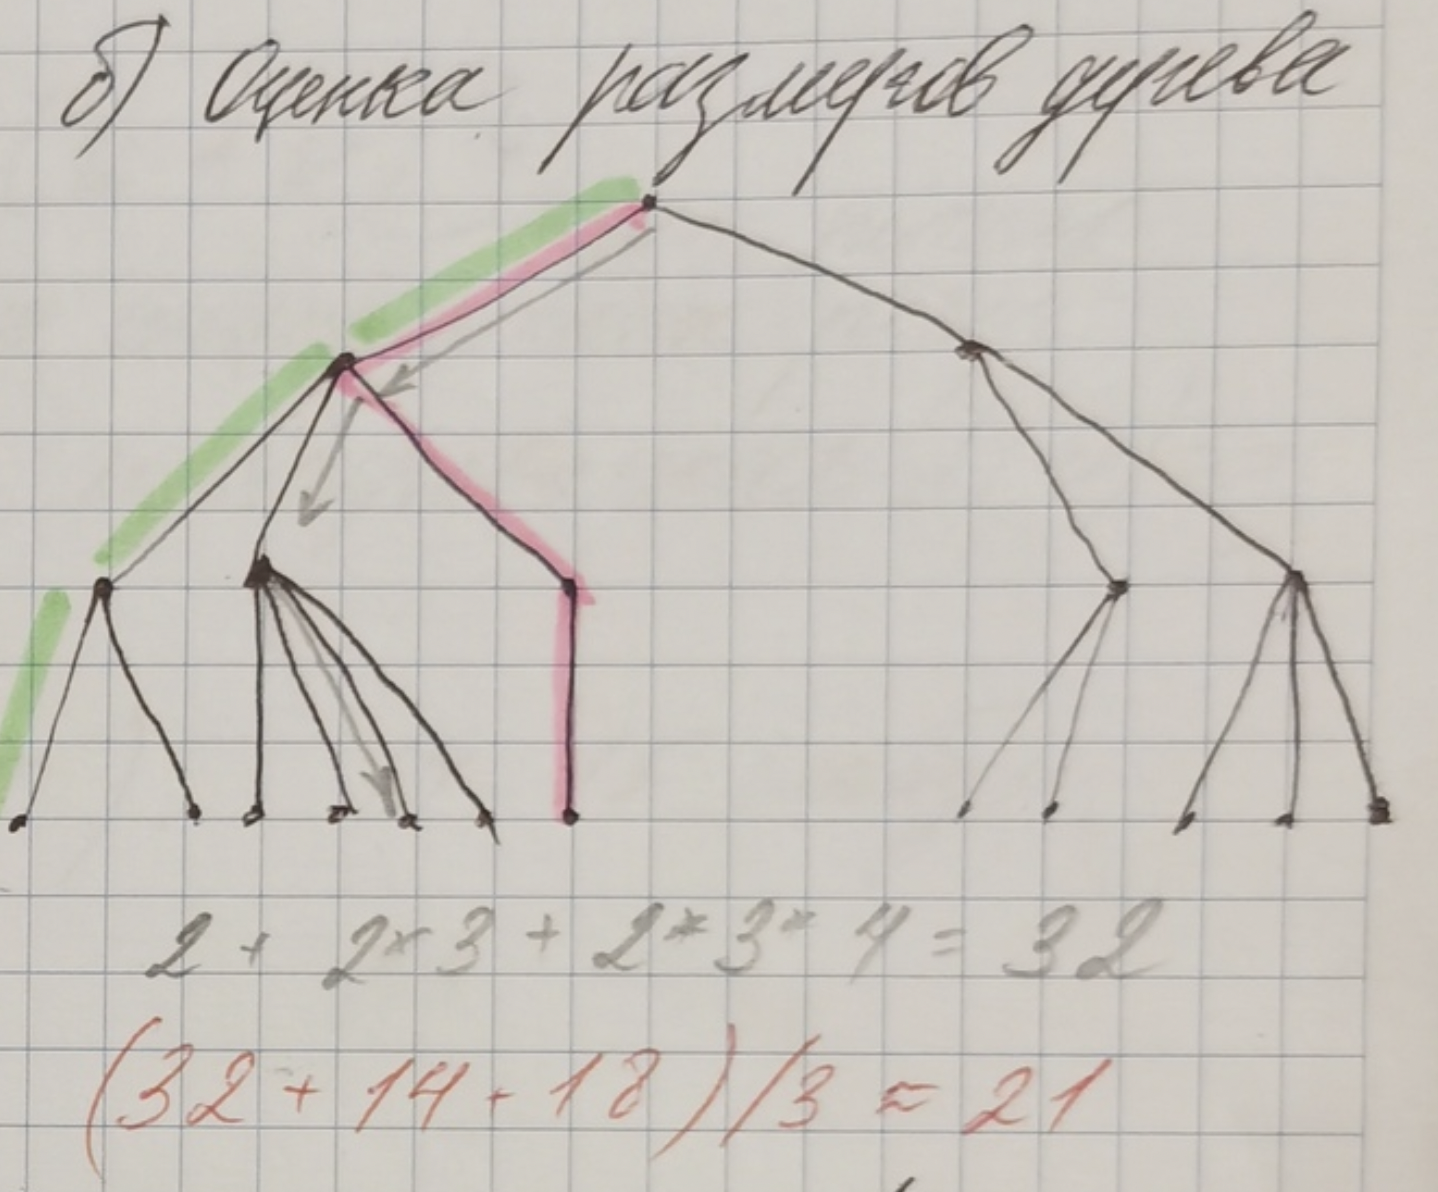
\includegraphics[width=0.5\textwidth]{images/chapter1/tree-size-example.png}
                \caption{Пример Калишенко метода Монте-Карло на размере дерева (на первой итерации, выделенной разноцветными маркерами, получили 32 узла, после чего по такой же схеме совершаем еще 2 итерации, в которых были получены 14 и 18 узлов)}
                \label{fig:images/chapter1/tree-size-example.png}
            \end{figure}

            \begin{center}
                $\ast$ \textbf{Ниже рассматриваются примеры, отличные от примера Калишенко, однако, также имеющих древовидную модель эксперемента.}
            \end{center}
        
            Предположим, у нас есть дерево решений для задачи принятия решений. Каждый узел дерева представляет собой определенное решение, а ребра дерева - возможные исходы или решения, которые могут быть приняты после каждого решения. Наша цель - оценить вероятность успеха задачи, то есть вероятность достижения конечного узла дерева, где считается, что задача успешно решена.

            Чтобы использовать метод Монте-Карло, мы можем случайным образом выбрать большое количество путей через дерево. Каждый путь представляет собой последовательность принятых решений, начиная с корневого узла и двигаясь по ребрам дерева, пока не достигнем конечного узла. Затем мы считаем, сколько из выбранных путей успешно решают задачу, и оцениваем вероятность успеха как отношение успешных путей к общему количеству выбранных путей.
            \\

            \bolditalic{Пример на крестиках-ноликах}\\
            Предположим, у нас есть дерево решений для игры в крестики-нолики. В корневом узле мы выбираем, кто будет ходить первым - крестики или нолики. Затем мы проходим через дерево, выбирая случайные ходы для каждого игрока, пока не достигнем конечного узла, представляющего окончательное состояние игры. Если в конечном узле игра выиграна крестиками, мы считаем путь успешным.\\

            \bolditalic{Еще пример (менее душный)}\\
            Из корня несколько раз случайным образом выбираем направления, по которым будем идти и после смотрим, является ли лист этого направления \textit{успешным} (В аналогии с площадью: \textit{Попали} или \textit{Не попали} в область). Так делаем $n$ раз, после чего считаем отношение \textit{Успешных Листьев} на $n$.
            
        
        \subsubsection{Пример на площади фигуры}

            Преположим, что надо вычислить площадь фигуры $S$, которая расположена внутри некоторого области (в данном случае - единичного квадрта).\\
            Выберем внутри этой области $N$ число случайных точек. Точки, попавшие в $S$ обозначим как $N^*$.\\\\
            Геометрически очевидно, что $\lim_{N \to \infty} \frac{N^*}{N}$ $= S$
            \begin{figure}[H]
                \centering
                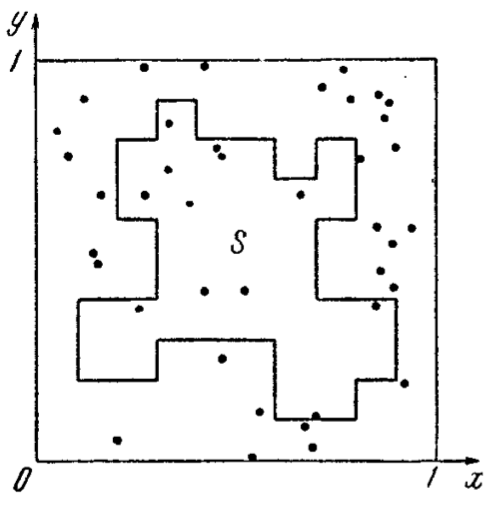
\includegraphics[width=0.2\textwidth]{images/chapter1/monte-carlo-area.png}
                \caption{Пример метода Монте-Карло на площади фигуры}
                \label{fig:images/chapter1/monte-carlo-area.png}
            \end{figure}
        
        \subsubsection{Ограничения и условия применимости}

            Чтобы применять метод Монте-Карло необходимо знать распределение в задачи, а также предел генерации случайных величин.\\

            Также, ошибка вычислений, как правило пропорциональная $\sqrt{\frac{D}{N}}$, где $D$ $-$ некоторая постоянная, а $N$ $-$ число испытаний.
        
\newpage
\section{Раскраска в 3 цвета}
    Source: \href{https://se.moevm.info/doku.php/courses:algorithms_building_and_analysis:materials:graph_coloring_notes#алгоритм_полного_перебора_совсем_наивный_перебор}{Конспект лекции по раскраскам}\\

    Когда говорят о раскраске графов, почти всегда подразумевают под этим раскраску их вершин, то есть присвоение цветовых меток вершинам графа так, чтобы любые две вершины, имеющие общее ребро, имели разные цвета. Другими словами, \bolditalic{необходимо найти правльную раскраску графа для 3-х цветов}.
    
    \subsection{Алгоритм полного перебора}

        Пусть дан граф и дана его раскраска. Чтобы проверить её корректность, нужно обойти все ребра и проверить, если одинаковые цвета на концах. Значит, сложность проверки - линейная.\\
    
        Самый простой вариант - генерация всех возможных три-раскрасок и проверка каждой на корректность. Сложность такого алгоритма - $O(3^n)$, т.к. это число возможных три-раскрасок графа.
    
    \subsection{Перебор с учётом выбора только из 2 цветов}
        Пусть есть некоторая вершина. Мы красим её в первый цвет. Для инцидентных вершин выбор идет не из 3-х цветов, а из 2-х. Сложность такого алгоритма - $O(2^n)$.\\

        Другими словами, используется знание, что инцидентные данной вершины нельзя красить в цвет данной.
    
    
    \subsection{Перебор подмножеств размера $\Longleftarrow$ $\frac{n}{3}$}

        Два соображения:
        \begin{enumerate}
            \item Если граф уже раскрашен, то вершины разделяются на множества - первого, второго и третьего цвета. Очевидно, что внутри этих множеств не существует ребер. Если есть $n$ вершин и 3 множества, очевидно, что одно из этих множеств будет иметь мощность $\leq \frac{n}{3}$ вершин.
            \item Пусть нам заранее известно одно из этих множеств. Если это так, то все оставшиеся вершины будут красится гораздо проще - с линейной сложностью.
        \end{enumerate}

        Значит, нужно найти такое множество. Способов выбрать такое множество:
        \begin{center}
            $ C_n^0 + C_n^1 + C_n^2 + ... + C_n^{\frac{n}{3}} \leq n * C_n^{\frac{n}{3}} \leq 1.9^n$ $-$ радиус шара Хэмминга.
        \end{center}

        Значит, сложность алгоритма $-$ $ O(1.9^n)$

    \subsection{Вероятностный алгоритм. Сведение к задаче выполнимости}

        Посмотрим все цвета для вершин, в которые можно их покрасить. Можно для каждой вершины случайным образом выкинуть один цвет и красить из оставшихся. В таком случае каждая вершина может быть покрасить в один из двух цветов.\\
    
        Такую задачу можно свести к \textbf{задаче выполнимости булевых формул (2SAT)}.\\
    
        Сведение такое:\\
    
        Пусть каждый цвет обозначается переменной $a_1, a_2, a_3$. Нужно покрасить все вершины в какие-то цвета. Это значит, что нужно выбрать хотя бы (и только) один из этих цветов. Т.е. для одной вершины верно следующее
        \begin{center}
            $(a_1 \vee a_2 \vee a_3) \wedge (\overline{a_1} \vee \overline{a_2}) \wedge (\overline{a_1} \vee \overline{a_3}) \wedge (\overline{a_2} \vee \overline{a_3})$
        \end{center}
        \textit{1-й дизъюнкт} - вершину нужно покрасить\\
        \textit{2, 3, 4-е дизъюнкты} - вершину можно покрасить только в один цвет.\\
    
        Ещё нужно учесть ограничение три-раскраски, т.е. добавить ограничение на неодинаковость цвета инцидентных вершин.
        \begin{center}
            $\wedge (\overline{a_1} \vee \overline{b_1}) \wedge (\overline{a_2} \vee \overline{b_2}) \wedge (\overline{a_3} \vee \overline{b_3})$
        \end{center}
        Вычеркнув неиспользуемые цвета получаем \textbf{задачу 2SAT}, где каждый дизъюнкт содержит не больше чем два литерала. Эту задачу можно решить за полиномиальное время.\\
    
        Задачу 2SAT возможно свести к графу, и решением будет поиск компонент связности.\\
    
        Если найдено решение задачи, то граф точно может быть раскрашен, но обратное неверно - возможно, мы вычеркнули нужные цвета для раскраски. Вероятность того, что раскраска выживет после вычеркивания $-$ $(\frac{2}{3})^n$. \textbf{Это очень мало}\\
        Но если прогнать алгоритм $(\frac{2}{3})^n$ раз, вероятность ошибки $-$ $\frac{1}{e}$\\
        Если после этого прогнать ещё $100$ раз, то вероятность ошибки $-$ $\frac{1}{e^{100}}$\\
        
        Сложность алгоритма $-$ $O(1.5^n)$
        
        \subsection{Применение раскраски на практике}
    
            \begin{enumerate}
                \item Задача планирования. Пусть есть список заказов, которые начинаются и заканчиваются в определенное время. Нужно понять, какое минимальное количество ресурсов нужно выделить для решения этих заказов. Сводится так: пересечение заказов по времени - ребро графа. Хроматическое число графа и есть ответ.
                \item Есть карта - отображение информации, которое предполагает, что между объектами есть границы (например - политическая карта мира). Задача - определить минимальное число цветов раскрасить карту, чтобы были видны границы между объектами. Задача очевидным образов сводится к раскраске графа.
                \item Задача оптимального распределения переменных по регистрам.
            \end{enumerate}
    
\newpage
\section{Задача коммивояжера}
    Source: \href{https://www.youtube.com/watch?v=r804FVgvaTo}{Лекция 1 | Алгоритмы для задачи коммивояжёра | Александр Куликов | Лекториум} \\
    
    Задача коммивояжера (Traveling Salesman Problem, TSP) является классической задачей оптимизации комбинаторного типа. В ней требуется найти самый короткий путь, проходящий через все заданные города и возвращающийся в исходный город. (Найти гамильтонов цикл минимальной длины)

    \subsection{Сложность полного перебора}

        Сложность полного перебора для задачи коммивояжера растет экспоненциально с увеличением количества городов.\\

        Предположим, у нас есть $N$ городов. Количество возможных путей для посещения всех городов и возврата в исходный город равно $(N-1)!$, поскольку первый город выбирается из $N$ возможных, второй - из оставшихся $N-1$ возможных и так далее, до последнего города, который автоматически определяется, так как остается только один непосещенный город.\\

        Таким образом, время выполнения полного перебора вариантов для задачи коммивояжера составляет $O((N-1)!)$, что является факториальной сложностью. Это означает, что с увеличением числа городов, время выполнения растет очень быстро и становится практически неосуществимым для больших $N$.
    
    \subsection{Метод ветвей и границ:}
        $\bullet$ Метод ветвей и границ (Branch and Bound) - это алгоритм для решения задачи коммивояжера и других комбинаторных задач оптимизации.\\

        $\bullet$  Основные две эвристики:
        \begin{enumerate}
            \item \textit{Ветви}: в каком порядке выбирать еще не посященные вершины (например, начинать с ближайших)
            \item \textit{Границы}: нижняя оценка на длину решений.\\
        \end{enumerate}

        $\bullet$ Особенности метода:
        \begin{enumerate}
            \item Находит оптимальное решение
            \item Время работы зависит и от эвристик, и от входных данных
        \end{enumerate}
        
        \subsubsection{Отсечка по текущему найденному пути}
            Если \textit{текущий} вес гамильтонова цикла больше, чем \textit{лучший вес} (нижняя оценка) - отсекаем ветку решений.
        
        \subsubsection{Отсечка по весу МОД}
        
            Вес оптимального цикла коммивояжера не меньше:
            \begin{enumerate}
                \item $\frac{1}{2} \sum_{v \in V} $ (два мин. ребра, смежных c $v$ )
                \item  веса минимального покрывающего дерева (при выкидывании ребра из оптимального цикла получается покрывающее дерево)
            \end{enumerate}
        
    \subsection{Локальный поиск}

        \begin{algorithm}
        \caption{Локальный поиск}
        \begin{algorithmic}
            \STATE $S \longleftarrow$ какое-нибудь начальное решение
            \WHILE{в окрестности $S$ есть решение $S^*$ большего веса}
                \STATE Заменить $S$ на $S^*$ 
            \ENDWHILE
            \RETURN{$S$}
        \end{algorithmic}
        \end{algorithm}
    
        \subsubsection{2-окружение}

            Суть: В каждом решение пытаемся стереть \textit{два ребра} и заменить на какие-нибудь другие.

            \begin{figure}[H]
                \centering
                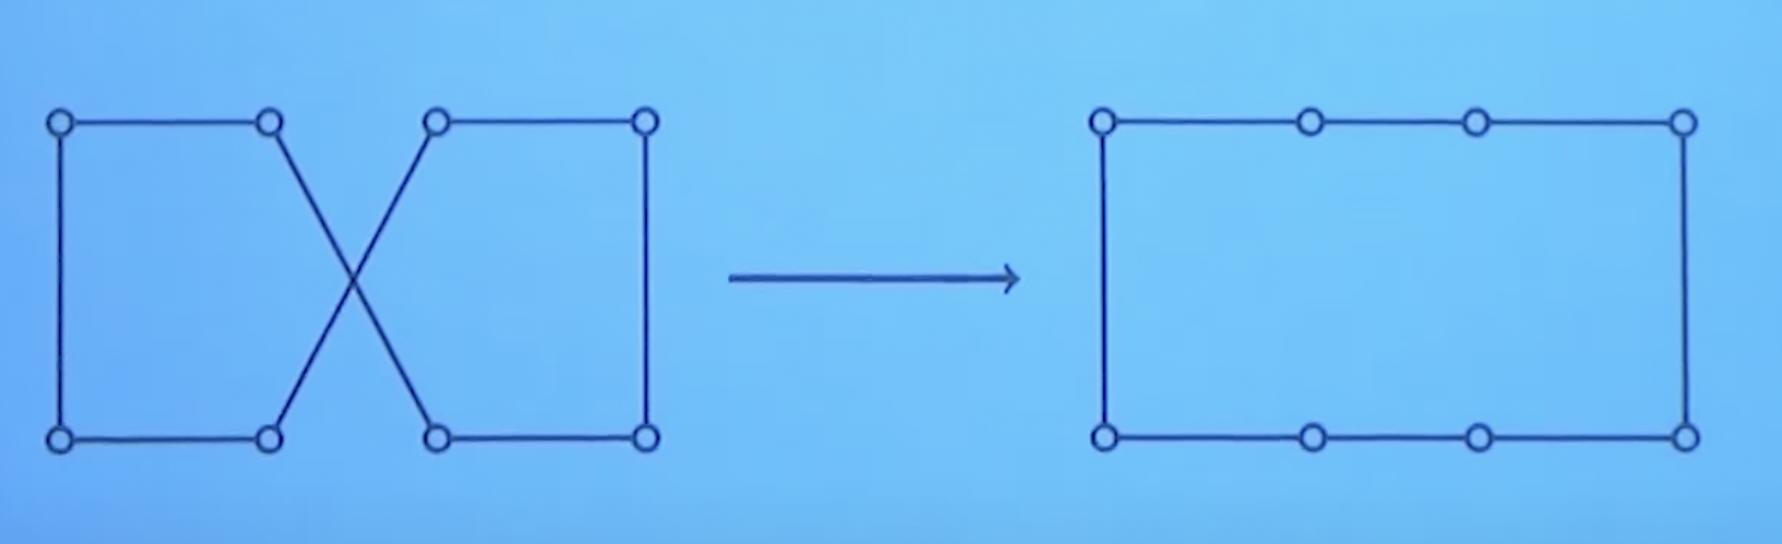
\includegraphics[width=0.6\textwidth]{images/chapter3/2-opt.png}
                \caption{2-окружение}
                \label{fig:images/chapter3/2-opt.png}
            \end{figure}
        
        \subsubsection{Имитация отжига}
            \begin{algorithm}
            \caption{Имитация отжига}
            \begin{algorithmic}
                \STATE $S \longleftarrow$ какое-нибудь начальное решение
                \LOOP
                    \STATE $S^* \longleftarrow$ случайное решение из окружения $S$
                    \STATE $\Delta \longleftarrow$ $cost(S^*) - cost(S)$
                    \IF{$\Delta < 0$}
                        \STATE заменить $S$ на $S^*$
                    \ELSE
                        \STATE заменить $S$ на $S^*$ с вероятностью $e^{\frac{-\Delta}{T}}$, где $T$ - температура или время
                    \ENDIF
                \ENDLOOP
            \end{algorithmic}
            \end{algorithm}

            \begin{figure}[H]
                \centering
                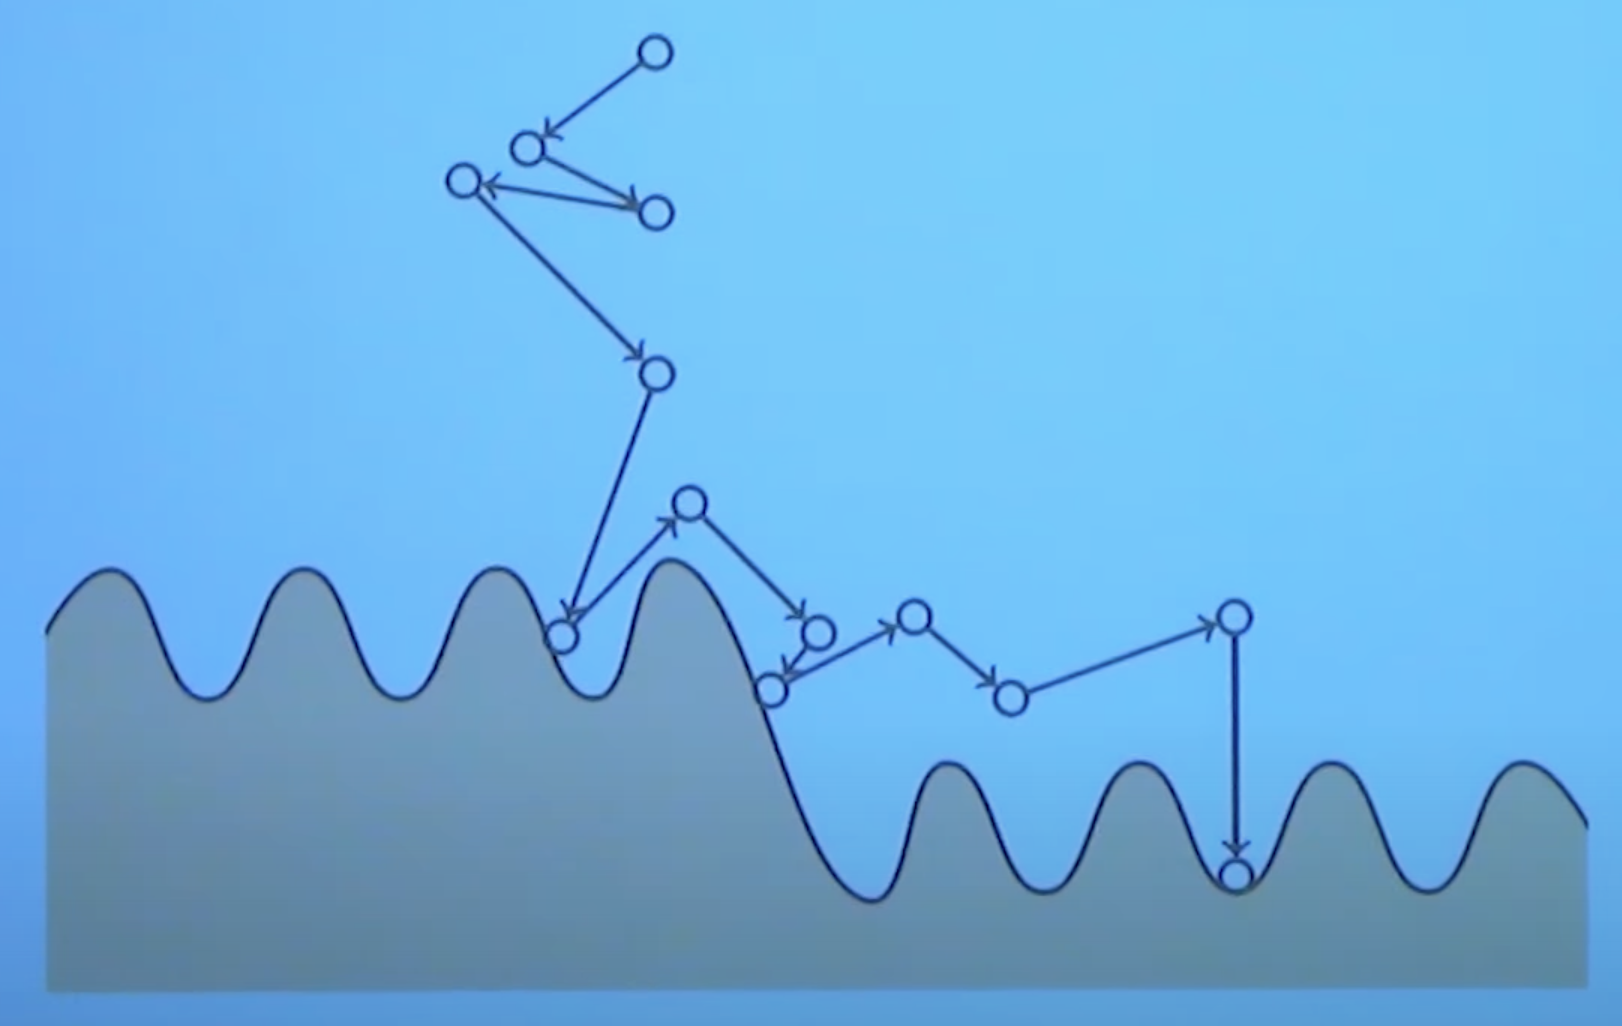
\includegraphics[width=0.8\textwidth]{images/chapter3/simulated-annealing-abstract.png}
                \caption{Метод имитации отжига абстрактно (выпрыгиваем из локального оптимума)}
                \label{fig:images/chapter3/simulated-annealing-abstract.png}
            \end{figure}
        
        
    \subsection{Приближённое решение (2-приближённый алгоритм)}

        $\ast$ \textbf{Коммивояжер в метрическом пространстве}:\\
        Частный случай для неориентированных графов, веса ребер которых удовлетворяют неравенству треугольника:
        \begin{center}
            $w(i,j) \leq w(i,k) + w(k,j)$
        \end{center}

        \begin{algorithm}
            \caption{2-приближенный алгоритм}
            \begin{algorithmic}
                \begin{enumerate}
                    \item Построить \textit{минимальное покрывающее дерево}(МОД) $T$
                    \item Продублировать каждое ребро дерева $T$
                    \item В полученном графе найти эйлеров цикл
                    \item Выкинуть из этого цикла все повторения вершин
                \end{enumerate}
            \end{algorithmic}
        \end{algorithm}

        \begin{proof}
         \begin{enumerate}
             \item Пусть $W_T$ $-$ вес МОД,  a $W_{opt}$ $-$ вес оптимального гамильтонова цикла.
             \item $W_T \leq W_{opt}$, поскольку при выкидывании ребра из гамильтонова цикла получается остовное дерево.
             \item Каждое ребро построенного гамильтонова цикла заменяет какой-то путь эйлерова цикла, длина которого по неравенству треугольника не менее длины этого ребра
             \item Значит, длина найденного пути не превосходит $2W_T$, а следовательно, и $2W_{opt}$
        \end{enumerate}   
        \end{proof}
            
    
\newpage
\section{Минимальный разрез в графе (Каргер-Штейн)}
    Source:
    \begin{enumerate}
        \item \href{https://neerc.ifmo.ru/wiki/index.php?title=Алгоритм_Каргера_для_нахождения_минимального_разреза}{Конспект ИТМО}
        \item $\ast$ \href{https://www.youtube.com/watch?v=ogodh2PQFug&t=23s}{Лекция 2 | Вероятностные алгоритмы | Иван Михайлин | Лекториум}
    \end{enumerate}

    \subsection{Примеры практических задач}
        
        
    \subsection{Алгоритм Каргера}
        \begin{definition}
            \textbf{Стягиванием} ребра $uv$ назовем последовательность действий:
            \begin{enumerate}
                \item Добавляем новую вершину $w$
                \item Для всех ребер $xu$ и $xv$ (где $x \in V$, $x \neq v$, $x \neq u$) добавляем новые ребра $xw$. При этом, если получаются кратные ребра $-$ оставляем их.
                \item Удаляем вершины $u$ и $v$ и все инцидентные им ребра.\\ 
            \end{enumerate}
        \end{definition}
        
        \begin{algorithm}
            \caption{Алгоритм Каргера}
            \begin{algorithmic}
                \STATE $minCut = \infty$
                \STATE $G = (V, E)$ // \textit{Некоторый граф с $V$ вершинами и $E$ ребрами}
                \STATE $i = 0$
                 \FOR{$i \leq n^2\ln{n}$}
                    \STATE $G^* = G$
                    \WHILE{$|V^*| > 2$}
                        \STATE Стягиваем случайное ребро из $G^*$
                    \ENDWHILE
                    \IF{$|E^*| < minCut$}
                        \STATE $minCut = |E^*|$
                    \ENDIF
                 \ENDFOR
            \end{algorithmic}
        \end{algorithm}\\

        Т.к. внутренний цикл ($while |V^*| > 2$) выполняется $n^2\ln{n}$ раз, то вероятность нахождения неверного ответа $\leq \frac{1}{n^2}$. Даже при небольших значениях $n$ алгоритм практически гарантированно выдает правильный ответ.\\

        $\bullet$ Оценка времени работы алгоритма\\
        Время работы внутреннего цикла $-$ $O(n^2)$, а внешнего $-$ $O(n^2\log(n))$, из чего следует, что время работы всего алгоритма $-$ $O(n^4\log(n))$.
        
        
        
    \subsection{Оптимизация Штейна алгоритма Каргера}
        $\times$ Будем называть внутренний цикл \textit{Аргоритма Каргера} функцией $GetCut$, а внешний $-$ функцией $MinCut$.\\

        $\bullet$ \textbf{Оптимизация заключается в следующем:}\\
        Заметим, что вероятность стягивания вершины, принадлежащей минимальному разрезу, в начале выполнения функции $GetCut$ довольно мала, в то время, как вероятность стянуть ребро, которое не следует стягивать, ближе к концу работы функции существенно возрастает. Тогда будем использовать следующую рекурсивную версию алгоритма:
        \begin{enumerate}
            \item Запускаем функцию $GetCut$ и стягиваем ребра до тех пор, пока не останется $\frac{n}{\sqrt{2}}$  вершин.
            \item Запускаем независимо эту же функцию для получившегося графа дважды и возвращаем минимальный из ответов.
        \end{enumerate}
        Такая модификация алгоритма выдает правильный ответ с точностью, не менее $\frac{1}{\log(n)}$. Время работы функции $GetCut$ вычисляется рекурсивной функцией:
        \begin{center}
            $T(n) =$ $O(n^2) + 2* T(\frac{n}{\sqrt{2}}) =$ $O(n^2\log(n))$
        \end{center}
        
        Это медленнее, чем оригинальный алгоритм, однако вероятность нахождения разреза минимального веса экспоненциально выше. Достаточно запустить алгоритм $c\log^2(n)$ раз, где $c$ $-$ некоторая константа. Действительно, рассчитаем вероятность неправильного ответа также, как раньше:
        \begin{center}
            $(1 - \frac{1}{\log(n))^{c\log^2(n)}}$ $\leq$ $e^{c\log^2(n) - \frac{1}{\log(n)}}$ $=$ $\frac{1}{n^c}$.
        \end{center}
        \textbf{Итоговое время работы} $-$ $O(n^2\log(n)) \cdot c\log^2(n)$ $=$ $O(n^2\log^3(n))$
        
        
        
\newpage
\section{Динамическое программирование}
%ТЕМУ БЕРЕТ ВОВА
    Динамическое программирование (DP) - это метод оптимизации, который позволяет решать задачи, разбивая их на более мелкие подзадачи и сохраняя результаты этих подзадач для последующего использования.
    
    \subsection{Примеры вычисления чисел Фибоначчи}
        Одна из классических задач, которую можно решить с использованием динамического программирования, - это вычисление чисел Фибоначчи. 
        Рассмотрим решение в лоб, а именно с помощью использования рекурсивной функции.
        \begin{lstlisting}[label=def-fibonacci-null-example,caption=Первый пример  вычисления чисел Фибоначчи рекурсией]
def fibonacci(n):
    if n==1:
        return 1
    else:
        return fibonacci(n-1)+fibonacci(n-2)
        \end{lstlisting}
        В чем недостаток данного метода. В том, что мы несколько раз будем пересчитывать одно и тоже значение, которое нами уже посчитано. Для этого и существует динамическое программирование, деление задачи на множество маленьких подзадач, единожды последовательно решив которые, мы получим результат. 
       \begin{lstlisting}[label=def-fibonacci-first-example,caption=Второй пример  вычисления чисел Фибоначчи Динамическим программированием]
def fibonacci(n):
    fib = [0, 1]

    for i in range(2, n + 1):
        fib.append(fib[i - 1] + fib[i - 2])

    return fib[n]
        \end{lstlisting}
    Главным недостатком данного подхода может показаться не рациональный расход памяти, однако этого можно заметить, что для вычисления следующего значения чисел фиббоначи, нам нужно 2 предыдущих, используем этот факт и получим следующий код.
    \begin{lstlisting}[label=def-update-fibonacci,caption=Примеры вычисления чисел Фибоначчи Динамическим программированием-2]
def fibonacci(n):
    prev_fib=0
    this_fib=1
    next_fib=0
    for i in range(2, n + 1):
        next_fib=this_fib+prev_fib
        prev_fib=this_fib
        this_fib=next_fib

    return next_fib
        \end{lstlisting}
        Такое решение имеет линейную сложность.
    \subsection{Редакционное расстояние}
    \begin{definition}
        \bolditalic{Расстояние Левенштейна (редакционное расстояние, дистанция редактирования)} $—$ метрика, измеряющая по модулю разность между двумя последовательностями символов. Она определяется как минимальное количество односимвольных операций (а именно вставки, удаления, замены), необходимых для превращения одной последовательности символов в другую.
        \begin{center}
            exponential  \\
            \times \times .. \updownarrow \updownarrow .+ \updownarrow \\
            potential 
        \end{center}
    \end{definition} 
    Здесь и далее будем рассматривать \times $-$ удаление, \updownarrow $-$ замена, + $-$ добавление.

    Решим эту задачу с помощью динамического программирования. 
    Введем функцию E(i,j), где i - первые i и j длины префиксов первой и второй строки.
    Тогда
    \begin{center}
        \begin{equation*}
        E(i,j) =min 
        \begin{cases}
         E(i-1,j)+1 &\text{вставка}\\
         E(i,j-1)+1 &\text{удаление}\\
         E(i-1,j-1)+diff(i,j) &\text{замена}
    \end{cases}
    \end{equation*}
    \begin{equation*}
    diff(i,j) = 
 \begin{cases}
   1 & i \neq j\\
   0 & i=j
 \end{cases}
\end{equation*}
    \end{center}
    Теперь если учесть, что  E(i,0) = i, а E(j,0)=j, то можно написать псевдокод.
    \begin{lstlisting}[label=def-reductio,caption=Пример  нахождения минимального количества операций преобразования одной строки в другую]
    def diff(i,j):
        if i==j:
            return 0
        else:
            return 1
    def count_operation_string(old_string,to_string,len_old_string,len_to_string):
        E = [[0] * len_old_string for i in range(len_to_string)]//инициализация
        for i in range(len_to_string)://первоночальное заполнение
            E[i][0]=i
        for j in range(len_old_string):
            E[0][j]=j
        for i in range(len_to_string)://проход по всем элементам массива.
            for j in range(len_old_string):
                E[i][j]=min(E[i-1][j]+1,E[i][j-1]+1,E[i-1][j-1]+diff(i,j))
        return E[len_old_string-1][len_to_string-1]
        \end{lstlisting}
    \subsection{Задача о порядке перемножения матриц}
    Сложность перемножения двух матриц O($n^3$)
    Рассмотрим пример перемножения трех матриц A(10\times 100), B(100\times 5), C(5\times 50).
    
    Количество итераций при:\\
    \begin{center}
        (A*B)*C=10*100*5+10*5*50=7500 итераций\\
        A*(B*C)=100*5*50+100*10*100=75000 итераций \\
    \end{center}
    Очевидно, что при изменении порядка перемножения матриц результат не изменится, а количество затраченных итераций на перемножения может быть разным.Возникает вопрос о таком перемножении матриц, при котором количество операций будет минимально, так как перемножение матриц сам по себе сложный процесс, имеющий кубическую сложность.\\
    Попробуем решить задачу с помощью динамического программирования.Введем функцию
     \begin{center}
        \begin{equation*}
        m[i,j] =
        \begin{cases}
         0 & i=j\\
         \underset{i<=k<j}{min}(m[i,k]+m[k+1,j]+p_{i-1}*p_{k}*p_{j} & i<j \\
        \end{cases}
    \end{equation*}
    \end{center}
    Будем обозначать произведение матриц $A_{i}*A_{i+1}..*A_{j-1}*A_{j}$ как $A_{i..j}$ .Данная функция обозначает минимальное количество операций скалярного умножения \\
    Тогда m[i,j] - минимальное количество скалярных умножений матриц $A_{i..j}$\\
    В этой формуле m[i,k]+m[k+1,j] уже перемноженные на предыдущих шагах матрицы $A_{i..k}, A_{k+1..j}$ 
    $p_{i-1}*p_{k}*p_{j}$ - это количество строк i-1 матрицы * количество столбцов k матрицы * количество столбцов j матрицы.\\
    p - это строка размерностей наших матриц. Для примера выше p=(10,100,5).\\
    Как нетрудно заметить, 1 элемент этого вектора - количесвто строк первой матрицы,последний элемент этого вектора - количество столбцов последней матрицы, а остальные элементы - количество строк правой и столбцов левой матрицы.
    
\newpage
\section{Поиск подстроки в строке (Кнут-Моррис-Пратт)}
    Source:
    \begin{enumerate}
        \item \href{https://neerc.ifmo.ru/wiki/index.php?title=Алгоритм_Кнута-Морриса-Пратта}{Алгоритм Кнута-Морриса-Пратта (ИТМО конспект)}
        \item \href{https://neerc.ifmo.ru/wiki/index.php?title=Префикс-функция}{Префикс-функция (ИТМО конспект)}
        \item \href{https://youtu.be/j51rfmaE1dY?t=342}{Лекция 5 | Алгоритмы в биоинформатике | Николай Вяххи | CSC | Лекториум}
    \end{enumerate}

    \subsection{Основные определения}
        \begin{definition}
            \bolditalic{Префикс функция} $-$ длина наибольшего префикса строки, которая не совпадает с этой строкой и одновременно является ее суффиксом:
            \begin{center}
                $S$ $=$ abacaba\\
                $P(S)$ $=$ 0010123
            \end{center}
        \end{definition}
    
    \subsection{Задача точного поиска образца в строке}
        Дана некоторая строка $pattern$ длины $n$ и строка $text$ длины $m$. Найти все вхождения $pattern$'а в $text$.
    
    \subsection{Наивный алгоритм и его сложность}
        Полный перебор всех элементов $text$, в котором сравниваются $pattern$ и $text[i:n]$.\\

        \textbf{Сложность} $-$ $O(n*m)$
    
    \subsection{Алгоритм КМП}
        Дана строка текста $T$ и шаблон $P$.\\
        Построим строку $S$ $=$ $P\#T$, где $\#$ $-$ любой символ, которого нету ни в $T$, ни в $P$. Посчитаем по ней значение префикс функции $p$. Из-за символа-разделителя выпонялется $\forall i :$ $p[i] \leq |P|$.\\
        Заметим, что по определению префикс-функции при $i > |P|$ и $p[i] = |P|$ подстроки длины $P$, начинающиеся с позиций $0$ и $i - |P| + 1$, совпадают.\\\\
        Соберем все такие позиции $i - |P| + 1$  строки $S$, вычтем из каждой позиции $|P| + 1$, это и будет ответ. Другими словами, если в какой-то позиции $i$ выполняется условие $p[i] = |P|$, то в этой позиции начинается очередное вхождение образца в цепочку.

        \begin{figure}[H]
                \centering
                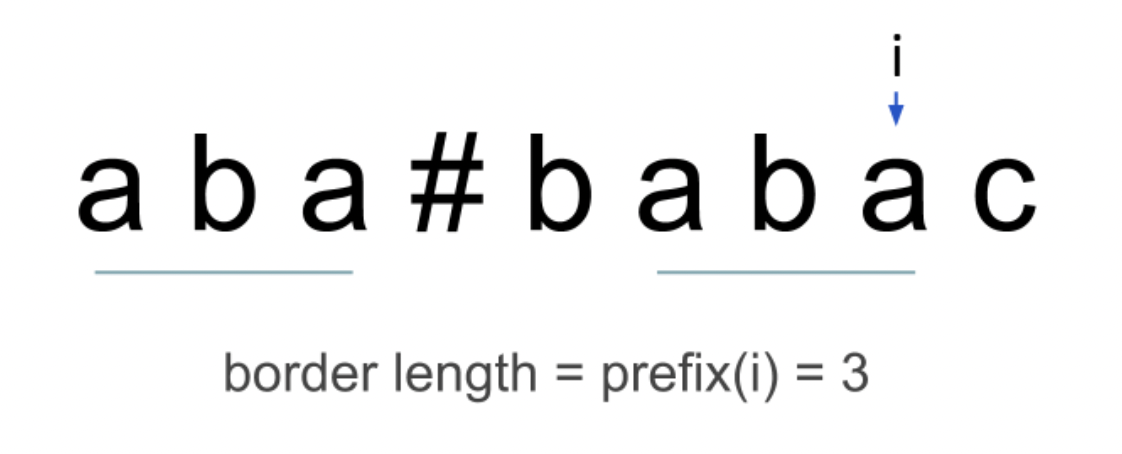
\includegraphics[width=0.5\textwidth]{images/chapter6/KMP.png}
                \label{fig:images/chapter6/KMP.png}
        \end{figure}
        
        \begin{algorithm}
        \caption{КМП}
            \begin{algorithmic}
                \STATE \textbf{int[]} kmp(string P, string T):
                \STATE \quad int pl = P.length
                \STATE \quad int tl = T.length
                \STATE \quad int[] answer
                \STATE \quad int[] p = prefixFunction(P + "\#" + T)
                \STATE \quad int count = 0
                \STATE \quad for i = 0 .. tl - 1
                \STATE \quad\quad if p[pl + i + 1] == pl
                \STATE \quad\quad\quad answer[count++] = i - pl
                \STATE \quad return answer
            \end{algorithmic}
        \end{algorithm}

        \textbf{Время работы}\\
        Префикс-функция от строки $S$ строится за $O(S) = O(P+T)$. Проход цикла по строке $S$ содержит $O(T)$ итераций. Итого, время работы алгоритма оценивается как $O(P+T)$
     
    \subsection{Наивное построение префикс-функции и его сложность}
        Наивный алгоритм вычисляет префикс-функцию непосредственно по определению, сравнивая префиксы и суффиксы строк. Обозначим длину строки за $n$. Будем считать, что префикс-функция хранится в массиве $p$.\\

        \begin{algorithm}
            \caption{Наивное построение префикс-функции}
            \begin{algorithmic}
                \STATE \textbf{int[]} prefixFunction(string s):
                \STATE \quad int[] p = int[s.length]
                \STATE \quad fill(p, 0)
                \STATE \quad \textbf{for} i = 0 to s.length - 1
                \STATE \quad\quad \textbf{for} k = 0 to i - 1
                \STATE \quad\quad\quad \textbf{if} s[0..k] == s[i - k..i]
                \STATE \quad\quad\quad\quad p[i] = k
                \STATE \quad \textbf{return} p
            \end{algorithmic}
        \end{algorithm}

        \textbf{Пример}\\
        Рассмотрим строку $abcabcd$, для которой значение префикс-функции равно $[0, 0, 0, 1, 2, 3, 0]$

        \begin{center}
            \begin{tabular}{c|c|c}
                \textbf{Шаг} & \textbf{Строка} & \textbf{Значение функции} \\
                \hline
                1 & a & 0 \\
                \hline
                2 & ab & 0 \\
                \hline
                3 & abc & 0 \\
                \hline
                4 & abca & 1 \\
                \hline
                5 & abcab & 2 \\
                \hline
                6 & abcabc & 3 \\
                \hline
                7 & abcabcd & 0 \\
                \hline
            \end{tabular}
        \end{center}
        
        \textbf{Время работы}\\
        Всего $O(n^2)$ итераций цикла, на каждой из который происходит сравнение строк за $O(n)$, что дает в итоге $O(n^3)$.
    
    \subsection{Построение префикс-функции за линейное время}
        Вносятся несколько важных замечаний:
        \begin{enumerate}[label=$\ast$]
            \item Заметим, что $p[i+1] \leq p[i] + 1$. Чтобы показать это, рассмотрим суффикс,оканчивающийся на позиции $i+1$  и имеющий длину $p[i+1]$, удалив из него последний символ, мы получим суффикс, оканчивающийся на позиции $i$ и имеющий длину $p[i+1] - 1$, следовательно неравенство $p[i+1] > p[i] + 1$ неверно.
            \item Избавимся от явных сравнений строк. Пусть мы вычислили $p[i]$, тогда, если $s[i+1] = s[p[i]]$, то $p[i+1] = p[i] + 1$.  Если окажется, что $s[i+1] \neq s[p[i]]$, то нужно попытаться попробовать подстроку меньшей длины. Хотелось бы сразу перейти к такому бордеру наибольшей длины, для этого подберем такое $k$, что $k = p[i] - 1$. Делаем это следующим образом. За исходное $k$ необходимо взять $p[i-1]$, что следует из первого пункта. В случае, когда символы $s[k]$ и $s[i]$ не совпадают, $p[k-1]$ $-$  следующее потенциальное наибольшее значениe $k$, что видно из рисунка. Последнее утверждение верно, пока $k > 0$, что позволит всегда найти его следующее значение. Если $k = 0$, то $p[i] = 1$ при $s[i] = s[1]$, иначе $p[i] = 0$.
        \end{enumerate}

        \begin{figure}[H]
                \centering
                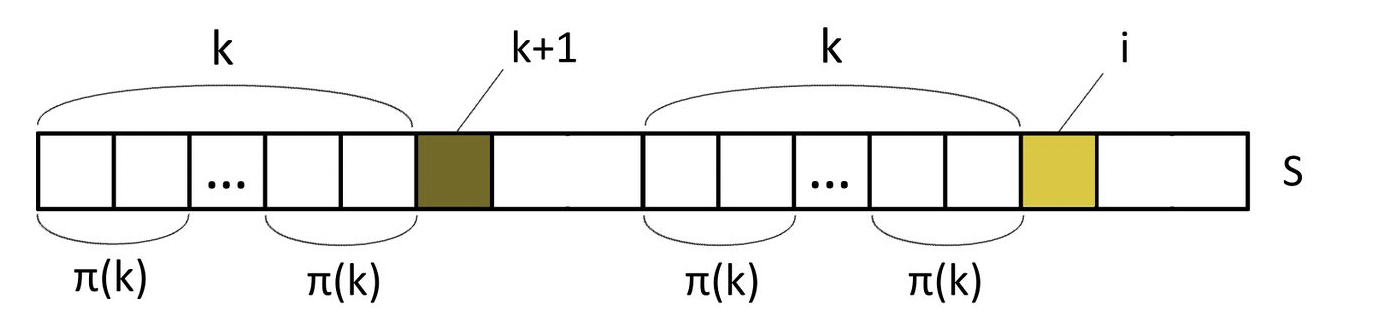
\includegraphics[width=0.8\textwidth]{images/chapter6/better_prefix_func.png}
                \label{fig:images/chapter6/better_prefix_func.png}
        \end{figure}

        \begin{algorithm}
        \caption{Эффективный алгоритм вычисления префикс-функции}
            \begin{algorithmic}
                \STATE \textbf{int[]} prefixFunction(string s):
                \STATE \quad int[] p = int[s.length]
                \STATE \quad p[0] = 0
                \STATE \quad \textbf{for} i = 1 to s.length - 1
                \STATE \quad\quad int k = p[i - 1]
                \STATE \quad\quad \textbf{while} k > 0 \textbf{and} s[i] != s[k]
                \STATE \quad\quad\quad k = p[k - 1]
                \STATE \quad\quad \textbf{if} s[i] == s[k]
                \STATE \quad\quad\quad k++
                \STATE \quad\quad p[i] = k
                \STATE \quad \textbf{return} p
            \end{algorithmic}
        \end{algorithm}

        \textbf{Время работы}\\
        Время работы алгоритма составит $O(n)$.\\

        Для доказательства этого нужно заметить, что итоговое количество итераций цикла $while$ определяет асимптотику алгоритма. Теперь стоит отметить, что $k$ увеличивается на каждом шаге не более чем на единицу, значит максимально возможное значение $k = n - 1$. Поскольку внутри цикла $while$ значение $k$ лишь уменьшается, получается, что $k$ не может суммарно уменьшиться больше, чем $n - 1$  раз. Значит цикл $while$ в итоге выполнится не более $n$ раз, что дает итоговую оценку времени алгоритма $O(n)$.
        
        

\newpage
\section{Поиск кратчайших путей. Эвристические алгоритмы}
    Source:
    \begin{enumerate}
        \item \href{https://se.moevm.info/doku.php/courses:algorithms_building_and_analysis:materials:shortest_ways}{Алгоритмы Дейкстра и Флойда-Уоршелла}
        \item \href{http://neerc.ifmo.ru/wiki/index.php?title=Алгоритм_A*}{Алгоритм A* (ИТМО конспект)}
        \item \href{https://neerc.ifmo.ru/wiki/index.php?title=Эвристики_для_поиска_кратчайших_путей}{Эвристики для поиска кратчайших путей (ИТМО конспект)}
        \item Для ATL, Reach, REALT, Иерархии путей, Arc flags использовал gpt, тк в интернете мало инфы, да и мне как-то лень сегодня
        \item $\ast$ \href{https://habr.com/ru/companies/2gis/articles/326638/}{Полезная статья на хабре про методы поиска мин пути в графе}
    \end{enumerate}
    \subsection{Алгоритм Дейкстры}
        \bolditalic{Алгоритм Дейкстры} находит кратчайший путь от одной из вершин графа до всех остальных. Алгоритм работает только для графов без рёбер отрицательного веса.\\

        \textbf{Идея алгоритма}
        \begin{enumerate}
            \item Каждый раз, когда мы хотим посетить новый узел, мы выберем узел с наименьшим известным расстоянием.
            \item Как только мы переместились в узел, мы проверяем каждый из соседних узлов. Мы вычисляем расстояние от соседних узлов до корневых узлов, суммируя стоимость ребер, которые ведут к этому новому узлу.
            \item Если расстояние до узла меньше известного расстояния, мы обновим самое короткое расстояние.
        \end{enumerate}
        На каждом шаге существует множество уже обработанных вершин и еще не обработанных.\\

        \begin{algorithm}
            \caption{Алгоритм Дейкстры}
            \begin{algorithmic}
                \FOR{$v \in V$}
                    \STATE $Dist[v] = \infty$
                    \STATE $Prev[v] = \emptyset$
                \ENDFOR

                \STATE $Dist[v' \in V] = 0$ // \textit{Стартовая вершина}
                \STATE // \textit{Первый шаг:}
                \STATE $H \longleftarrow MakeQueue()$ // \textit{формирование очереди с приоритетами для вершины $v'$. Все инцидентные вершины попадают сюда}
                \WHILE{$H \neq \emptyset$}
                    \STATE $v \longleftarrow min(H)$ // \textit{из очереди с приоритетами выбирается минимальный $Dist[v]$}
                    \FOR{$vu \in E$ // \textit{для каждого инцидентного ребра} }
                        \IF{$(Dist[u] > Dist[v] + w(v,u)$ // \textit{если расстояние до вершины больше, чем то, по которому мы проходим - условие релаксации}}
                            \STATE $Dist[u] \longleftarrow Dist[v] + w(v,u)$
                            \STATE $Prev[u] \longleftarrow UpdatePriorities(H)$
                        \ENDIF
                    \ENDFOR
                \ENDWHILE
            \end{algorithmic}
        \end{algorithm}
        
        \textbf{Сложность алгоритма}\\
        Худший случай - каждый путь содержит в себе все остальные ( $v$ вершин). Если каждый такой путь будет хранится к каждой вершине, память будет $v^2$. Для оптимизации в каждой вершине хранится не весь путь, а только предыдущую вершину, из которой можно попасть в текущую.\\

        Общая сложность алгоритма:
        \begin{enumerate}
            \item $O(v^2)$ $-$ при работе на массиве;
            \item $O(\ln(v))$ $-$ при работе на куче.
        \end{enumerate}
        Если количество ребер небольшое, выгоднее использовать реализацию на куче, если же ребер намного больше, чем вершин, лучше использовать работу на массиве.\\

        \textbf{Применение алгоритма}\\
        Одно из применений алгоритма - маршрутизация. Например, алгоритм OSPF (Open Shortest Pass First). Каждый маршрутизатор строит некоторый граф и использует алгоритм Дейкстры в чистом виде.

        
    \subsection{A*}
        \bolditalic{Алгоритм поиска A*} — относится к эвристическим алгоритмам поиска по первому лучшему совпадению на графе с положительными весами ребер, который находит маршрут с наименьшей стоимостью от одной вершины (начальной) к другой (целевой, конечной).\\
        Алгоритм использует вспомогательную функцию (эвристика), чтобы направлять поиск решения и сокращать его длительность. Алгоритм полный в том смысле, что всегда находит оптимальное решение, если он существует.\\

        \textbf{Описание алгоритма}\\
        В процессе работы алгоритма для вершин рассчитывается функция $f(v)$ $=$ $g(v)$ $+$ $h(v)$, где
        \begin{enumerate}
            \item $g(v)$ $-$ наименьшая стоимость пути в $v$ из стартовой вершины,
            \item $h(v)$ $-$ эвристическое приближение стоимости пути от $v$ до конечной цели.
        \end{enumerate}
        Фактически, функция $f(v)$ — длина пути до цели, которая складывается из пройденного расстояния $g(v)$ и оставшегося расстояния $h(v)$. Исходя из этого, чем меньше значение $f(v)$,  тем раньше мы откроем вершину $v$ , так как через неё мы предположительно достигнем расстояние до цели быстрее всего. Открытые алгоритмом вершины можно хранить в очереди с приоритетом по значению $f(v)$. \textbf{$A*$} действует подобно алгоритму Дейкстры и просматривает среди всех маршрутов ведущих к цели сначала те, которые благодаря имеющейся информации (эвристическая функция) в данный момент являются наилучшими.

        \begin{definition}
            Говорят, что эвристическая оценка $h(v)$ \textbf{допустима} , если для любой вершины $v$ значение $h(v)$ меньше или равно весу кратчайшего пути от $v$ до цели.
        \end{definition}
        Допустимая оценка является оптимистичной, потому что она предполагает, что стоимость решения меньше, чем оно есть на самом деле.
        Второе, более сильное условие — функция $h(v)$ должна быть \textbf{монотонной} (т.е для любой вершины $v_1$ и ее потомка $v_2$ разность $h(v_1)$ и $h(v_2)$ не превышает фактического веса ребра $c(v_1, v_2)$ от $v_1$ и $v_2$, а эвристическая оценка целевого состояния равна нулю).\\

        \textbf{Реализация}
        \begin{enumerate}
                \item $Q$ $-$ множество вершин, которые требуется рассмотреть,
                \item $U$ $-$ множество рассмотренных вершин,
                \item $f[x]$ $-$ значение эвристической функции "расстояние + стоимость" для вершины $x$,
                \item $g[x]$ $-$ стоимость пути от начальной вершины до $x$,
                \item $h(x)$ $-$ эвристическая оценка расстояния от вершины $x$ до конечной вершины.
        \end{enumerate}
        На каждом этапе работы алгоритма из множества $Q$ выбирается вершина с наименьшим значением эвристической функции и просматриваются её соседи. Для каждого из соседей обновляется расстояние, значение эвристической функции и он добавляется в множество $Q$.
        \begin{algorithm}
            \caption{A*}
            \begin{algorithmic}
                \STATE $U = \emptyset$
                \STATE $Q = \emptyset$
                \STATE $Q.push(start)$
                \STATE $g[start] = 0$
                \STATE $f[start] = g[start] + h(start)$
                \WHILE{$Q.size() \neq 0$}
                    \STATE $current = $ вершина из $Q$ с минимальным значением $f$
                    \IF{$current = goal$}
                        \RETURN{Нашли путь до нужной вершины}
                    \ENDIF

                    \STATE $Q.remove(current)$
                    \STATE $U.push(current)$
                    \FOR{$v$ $:$  смежных с current вершины}
                        \STATE $tentativeScore = g[current] + d(current, v) $ // \textit{d(current, v) — стоимость пути между current и v}
                        \IF{$v \in U$ \textbf{and} $tentativeScore \geq g[v]$}
                            \STATE \textbf{continue}
                        \ENDIF
                        \IF{$v \notin U$ \textbf{or} $tentativeScore < g[v]$}
                            \STATE $parent[v] = current$
                            \STATE $g[v] = tentativeScore$
                            \STATE $f[v] = g[v] + h(v)$
                            \IF{$v \notin Q$}
                                \STATE $Q.push(v)$
                            \ENDIF  
                        \ENDIF
                    \ENDFOR
                \ENDWHILE
            \end{algorithmic}
        \end{algorithm}\\

        \textbf{Примеры эвристик}:
        \begin{enumerate}
            \item Если мы можем перемещаться в четырех направлениях, то в качестве эвристики стоит выбрать \bolditalic{манхэттенское расстояние}
                \begin{center}
                    $h(v)$ $=$ $|v.x - goal.x| + |v.y - goal.y|$
                \end{center}
            \item \bolditalic{Расстояние Чебышева} применяется, когда к четырем направлениям добавляются диагонали:
                \begin{center}
                    $h(v)$ $=$ max($|v.x - goal.x|, |v.y - goal.y|$)
                \end{center}
            \item Если передвижение не ограничено сеткой, то можно использовать \bolditalic{евклидово расстояние} по прямой:
                \begin{center}
                    $h(v)$ $=$ $\sqrt{(v.x - goal.x)^2 + (v.y - goal.y)^2}$
                \end{center}
        \end{enumerate}
    
    \subsection{ALT}
        \bolditalic{Алгоритм ATL} (A* + Landmarks + Triangle inequality) - это комбинированный алгоритм поиска кратчайшего пути, который объединяет идеи из трех различных подходов: алгоритма A* (A-star), использования ориентиров (landmarks) и неравенства треугольника.\\
        \textit{Ориентиры} $-$ это ключевые вершины графа, выбранные для вычисления приближенных расстояний до остальных вершин.\\

        \textbf{Вот основные шаги алгоритма ATL}:
        \begin{enumerate}
            \item \bolditalic{Подготовка данных}: Перед началом поиска кратчайшего пути производится предварительная обработка графа. Это может включать в себя определение ориентиров (landmarks) - ключевых вершин, для которых будут вычислены расстояния до всех остальных вершин.
            \item \bolditalic{Вычисление расстояний до ориентиров}: Используя выбранные ориентиры, вычисляются приближенные расстояния от каждой вершины графа до каждого ориентира. Это можно сделать с помощью алгоритма поиска кратчайшего пути, такого как алгоритм Дейкстры.
            \item \bolditalic{Вычисление нижних оценок}: На основе полученных приближенных расстояний строятся нижние оценки расстояний от каждой вершины до целевой вершины. Это выполняется путем комбинирования приближенных расстояний до ориентиров с использованием неравенства треугольника, чтобы получить наиболее оптимистичные оценки.\\
            Будем использовать неравенство треугольника для нижних оценок пути. Пусть $A$ $-$ один из ориентиров, тогда:
            \begin{enumerate}[label={$\cdot$}]
                \item $dist(v, w)$ $\geq$ $dist(A, w) - dist(A, v)$
                \item $dist(v, w)$ $\geq$ $dist(v, A) - dist(w, A)$
                \item $dist(v, w)$ $\geq$ max$\{ dist(A, w) - dist(A, v), dist(v, A) - dist(w, A)\}$
            \end{enumerate}
            \item \bolditalic{Использование A*}: Запускается алгоритм A* для поиска кратчайшего пути от исходной вершины к целевой. При этом для выбора следующей вершины используются нижние оценки, вычисленные на предыдущем шаге.
            \item \bolditalic{Повторение процесса}: Если алгоритм A* не достиг целевой вершины, можно повторить шаги 2-4, чтобы улучшить оценки и продолжить поиск пути.\\
        \end{enumerate}

        Алгоритм ATL пытается улучшить производительность алгоритма A* путем использования ориентиров и неравенства треугольника для получения более точных и оптимистичных оценок расстояний. Это позволяет ускорить поиск пути, особенно в больших графах или в случаях с длинными путями.
    
    \subsection{Reach}
        \bolditalic{Алгоритм Reach} (или Reachability Algorithm) - это алгоритм, используемый для определения достижимости между вершинами в ориентированном графе. Его основная цель - определить, можно ли достичь одну вершину из другой по заданному направлению ребер.\\

        \textbf{Основные шаги алгоритма Reach}:
        \begin{enumerate}
            \item \bolditalic{Инициализация}: Устанавливаются начальные значения для каждой вершины графа. Обычно все вершины помечаются как недостижимые.
            \item \bolditalic{Установка начальных вершин}: Выбирается начальная вершина или группа вершин, для которых будем искать достижимость. Это может быть одна вершина или набор вершин, в зависимости от требуемых условий.
            \item \bolditalic{Обход графа}: Начиная с выбранных начальных вершин, выполняется обход графа с помощью поиска в глубину (DFS) или поиска в ширину (BFS). При обходе графа помечаются достижимые вершины.
            \item \bolditalic{Проверка достижимости}: После завершения обхода графа проверяется, достижимы ли целевые вершины из выбранных начальных вершин. Если достижимость обнаружена, соответствующие вершины помечаются как достижимые.
            \item \bolditalic{Завершение}: Алгоритм Reach завершается после проверки достижимости целевых вершин и обновления их меток.
        \end{enumerate}\\

        Алгоритм Reach широко используется для определения достижимости и проверки связности в графах. Он может быть применен в различных областях, включая анализ социальных сетей, оптимизацию маршрутов и выявление взаимосвязей в данных.
    
    \subsection{REALT}
        Основная идея алгоритма REALT заключается в поиске кратчайшего пути от целевой вершины к исходной вершине, в то время как большинство классических алгоритмов поиска пути ищут путь от исходной вершины к целевой. Алгоритм REALT работает в обратном направлении, начиная с целевой вершины и двигаясь к исходной.\\

        \textbf{Основные шаги алгоритма REALT}:
        \begin{enumerate}
            \item \bolditalic{Инициализация}: Устанавливаем расстояние до целевой вершины равным нулю, а расстояние до остальных вершин - бесконечностью.
            \item \bolditalic{Установка приоритетов}: Для каждой вершины графа вычисляем приоритет, который определяется как минимальное расстояние от данной вершины до целевой вершины.
            \item \bolditalic{Итерации}: В каждой итерации выбираем вершину с наибольшим приоритетом и обновляем расстояния до ее соседей. Если новое расстояние меньше текущего, обновляем его.
            \item \bolditalic{Завершение}: Повторяем итерации до тех пор, пока не достигнем исходной вершины или пока все вершины не будут обработаны.
            \item \bolditalic{Восстановление пути}: Если мы достигли исходной вершины, восстанавливаем кратчайший путь, используя информацию о предыдущих вершинах.
        \end{enumerate}\\

        Алгоритм REALT имеет преимущества в скорости работы и потребляемых ресурсах для больших графов. Однако он может быть ограничен использованием только взвешенных ориентированных графов и не является универсальным для всех типов графов.
    \subsection{Иерархии путей}
        \bolditalic{Алгоритм Иерархии путей} (Pathfinding Hierarchy Algorithm) $-$ это алгоритм поиска кратчайшего пути в графе с использованием предварительной обработки иерархической структуры.\\

        \textbf{Основаня идея}\\
        Основная идея алгоритма Иерархии путей заключается в разделении графа на несколько уровней или слоев, где каждый уровень представляет собой абстракцию вершин более низкого уровня. Таким образом, граф становится иерархическим, где вершины на более высоких уровнях объединяют группы вершин на более низких уровнях.\\

        \textbf{Основные шаги}:
        \begin{enumerate}
            \item \bolditalic{Построение иерархии}: Исходный граф разбивается на уровни или слои. Это может быть достигнуто различными способами, например, с помощью кластеризации вершин или использования методов снижения размерности.
            \item \bolditalic{Предварительная обработка}: Для каждого уровня графа вычисляются кратчайшие пути между всеми парами вершин на этом уровне. Это можно сделать с помощью любого эффективного алгоритма поиска пути, например, алгоритма Дейкстры или алгоритма A*.
            \item \bolditalic{Поиск пути}: Для поиска кратчайшего пути между исходной и целевой вершинами используется иерархический подход. Сначала находятся ближайшие вершины на высоком уровне, затем на следующем более низком уровне, и так далее. Затем выполняется поиск пути на каждом уровне, используя предварительно вычисленные кратчайшие пути.
            \item \bolditalic{Комбинирование путей}: Когда кратчайшие пути найдены на каждом уровне, они комбинируются для получения общего кратчайшего пути между исходной и целевой вершинами. Это может быть достигнуто с помощью слияния путей на разных уровнях и устранения дублирования вершин.
        \end{enumerate}\\

        Алгоритм Иерархии путей позволяет ускорить поиск кратчайшего пути за счет использования предварительной обработки и разделения графа на более простые уровни. Он особенно полезен для

    
    \subsection{Arc flags}
        \bolditalic{Алгоритм Arc-Flag} $-$ это эффективный алгоритм для поиска минимального пути в графе, основанный на использовании специальных флагов (arc flags) на ребрах графа. Он позволяет сократить количество обрабатываемых ребер и ускорить поиск минимального пути.\\

        \textbf{Основные шаги}:
        \begin{enumerate}
            \item \bolditalic{Предварительная обработка}: Для каждого ребра в графе вычисляются и сохраняются дополнительные данные, такие как вес ребра или другая информация, необходимая для определения минимального пути.
            \item \bolditalic{Установка флагов на ребрах}: На некоторых ребрах графа устанавливаются флаги, которые указывают на определенные свойства ребер. Флаги могут отражать различные характеристики ребер, например, наличие определенных ограничений или особенностей.
            \item \bolditalic{Поиск пути}: Алгоритм выполняет поиск минимального пути от одной вершины графа к другой, используя флаги и предварительно вычисленные данные о ребрах. При поиске пути алгоритм учитывает только те ребра, на которых установлены соответствующие флаги.
            \item \bolditalic{Обновление флагов}: По мере продвижения вдоль пути алгоритм обновляет флаги на ребрах в соответствии с посещенными вершинами и другой информацией о пути. Это может включать установку или снятие флагов в зависимости от изменений в пути или посещенных вершинах.
            \item \bolditalic{Оптимизация и повторный поиск}: После завершения первого поиска пути алгоритм может проанализировать результаты и выполнить дополнительные оптимизации, например, сократить количество флагов или переиспользовать предварительно вычисленные данные. Затем может быть выполнен повторный поиск пути для получения окончательного минимального пути.
        \end{enumerate}\\

        Алгоритм Arc-Flag позволяет существенно сократить количество ребер, которые требуется рассмотреть при поиске минимального пути, путем использования флагов и выборочной обработки только некоторых ребер. Это делает его эффективным в случаях, когда графы очень большие или имеют большое количество ребер, и позволяет достичь более быстрых временных характеристик алгоритма поиска минимального пути.
    

\newpage
\section{Максимальный поток в графе. Алгоритм проталкивания предпотока}
    Source:
    \begin{enumerate}
        \item \href{https://neerc.ifmo.ru/wiki/index.php?title=Метод_проталкивания_предпотока}{Метод проталкивания предпотока (ИТМО конспект)}
        \item \href{https://vec.etu.ru/moodle/mod/resource/view.php?id=154630}{Запись лекции "Алгоритм Гольдберга"}
        \item $\ast$ \href{https://www.youtube.com/watch?v=knZXYrKYYbI}{Лекция 1 | Избранные главы теории потоков | Максим Бабенко | Лекториум}
        \item $\ast$ \href{https://www.youtube.com/watch?v=Na8jHUJtbYY}{Лекция 4 | Избранные главы теории потоков | Максим Бабенко | Лекториум}
        \item $\ast$ \href{https://www.youtube.com/watch?v=hYsVDmGaxkQ}{Лекция 5 | Избранные главы теории потоков | Максим Бабенко | Лекториум}
    \end{enumerate}
    \subsection{Идея push-relabel алгоритмов}
        Для понимания идеи алгоритма представим, что наша сеть — система из резервуаров, находящихся на определенной высоте, и соединяющих их труб с заданными пропускными способностями, соответствующих вершинам и рёбрам в исходной сети. Сам алгоритм можно представить как процесс поочередного "переливания" жидкости (операция проталкивания) из одного резервуара в другие, находящиеся на меньшей высоте, до тех пор пока не перестанет существовать резервуар, соответствующий переполненной вершине. Может случиться ситуация, что все трубы, выходящие из переполненной вершины $u$, ведут к вершинам, находящимся на такой же высоте что и $u$ или выше её. В таком случае поднимем резервуар (операция подъёма), соответствующий данной вершине, таким образом, чтобы его высота стала на единицу больше, чем высота самого низкого из смежных резервуаров. После подъёма будет существовать по крайней мере одна труба, по которой можно пропустить жидкость.\\
    
        В итоге, у нас не останется ни одной переполненной вершины, та часть потока, которая могла пройти к стоку, окажется там, остальная же вернется в исток. В такой ситуации предпоток превращается в обычный поток, так как для каждой вершины выполняется условие сохранения потока. Как будет показано далее, предпоток становится не только обычным, но и максимальным потоком.
    
    \subsection{Формализмы и инварианты}

    \begin{definition}
        \textbf{Предпотоком} (Preflow) будем называть функцию $f:V\times V\rightarrow \mathbb{R}$, удовлетворяющую следующим свойствам:
        \begin{enumerate}
            \item $f(u,v)=-f(v,u)$ (антисимметричность)
            \item $f(u,v)\leq c(u,v)$ (ограничение пропускной способностью)
            \item $\forall u\in V\setminus\{s,t\}, \sum\limits_{v\in V} f(v,u)\geq 0$ (ослабленное условие сохранения потока)
        \end{enumerate}
        $\ast$ Как можно заметить, по своим свойствам предпоток очень похож на поток и отличается лишь тем, что для него не выполняется закон сохранения потока.
        
    \end{definition}

    \begin{definition}
        \textbf{Избыточным потоком}, входящим в вершину $u$, назовем величину $e(u)=\sum\limits_{v\in V} f(v,u)$.\\ Тогда вершина $u\in V\setminus\{s,t\}$ будет называться \textbf{переполненной}, если $e(u)>0$.
    \end{definition}
    \begin{figure}[H]
                \centering
                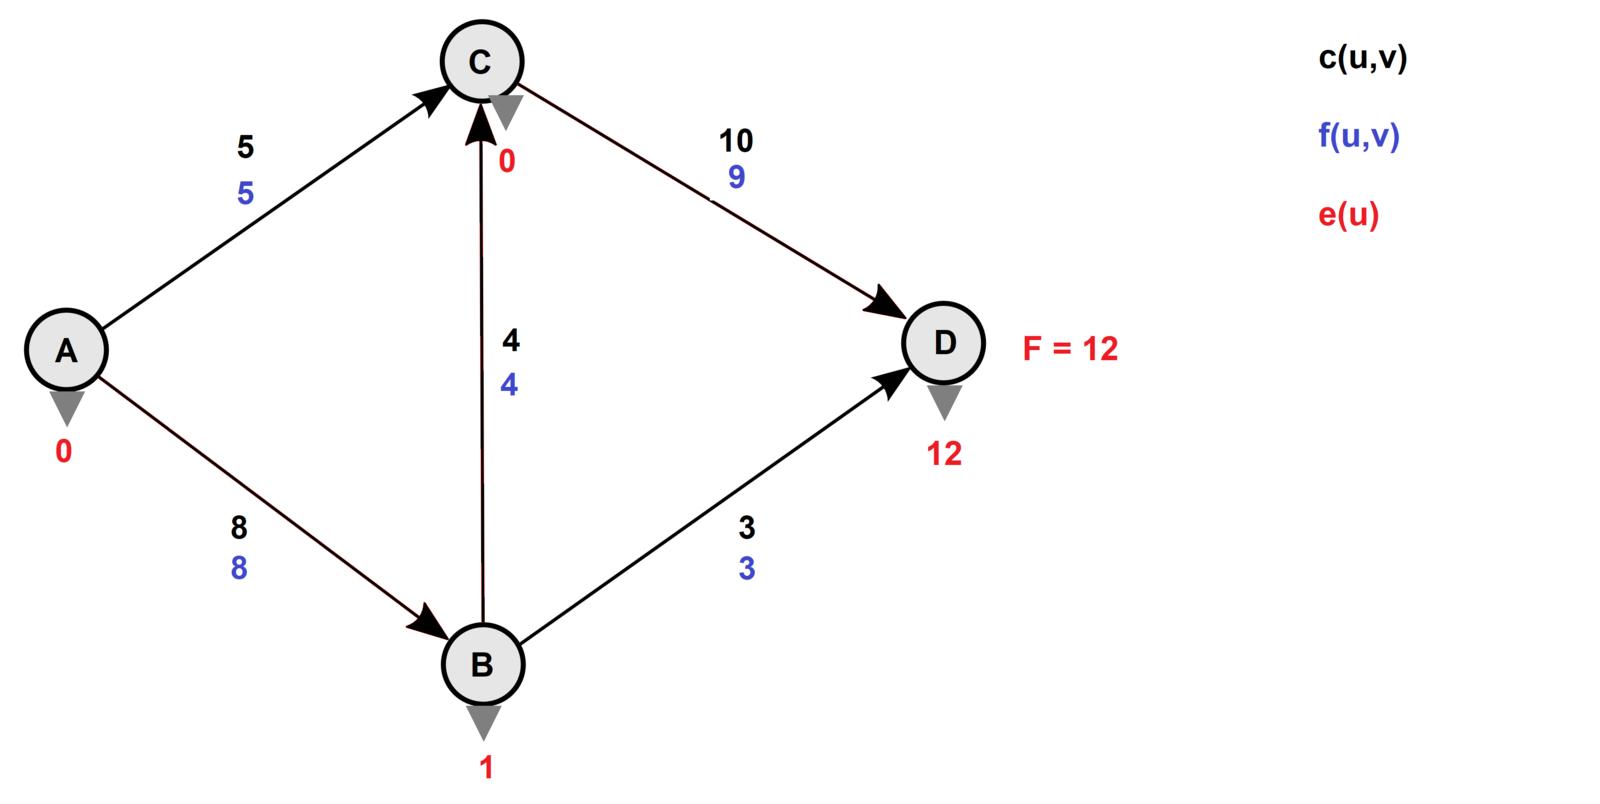
\includegraphics[width=0.6\textwidth]{images/chapter8/OrGraphExample.png}
                \caption{Пример сети с истоком A и стоком D. Вершина B является переполненной.}
                \label{fig:images/chapter8/OrGraphExample.png}
    \end{figure}

    \begin{definition}
        Функция $h:V\rightarrow \mathbb{Z}^+$ называется \textbf{высотой вершины}, если она удовлетворяет условиям:
        \begin{enumerate}
            \item $h(s)=|V|$
            \item $h(t)=0$
            \item $\forall (u,v)\in E, h(u)\leq h(v)+1$
        \end{enumerate}
        \hline
    \end{definition}\\

    $\bullet$ \textbf{Проталкивание (push)}\\
    Операция проталкивания из вершины $u$ в вершину $v$ может применяться тогда, когда $e(u)>0$, то есть вершина $u$ является переполненной, $c_f(u,v)>0$ и $h(u)=h(v)+1$.\\

    Данная операция работает следующим образом: по ребру $(u,v)$ пропускается максимально возможный поток, то есть минимум из избытка вершины $u$ и остаточной пропускной способности ребра $(u,v)$, вследствие чего избыток вершины $u$, остаточная пропускная способность ребра $(u,v)$ и поток по обратному ребру $(v,u)$ уменьшаются на величину потока, а избыток вершины $v$, поток по ребру $(u,v)$ и остаточная пропускная способность обратного ребра $(v,u)$ увеличиваются на эту же величину.

    \begin{algorithm}
    \caption{Push Function}
        \begin{algorithmic}
        \STATE \textbf{Function} push(\textbf{Node} $u$, \textbf{Node} $v$)
            \STATE \quad \quad $d = \min(e(u), c(u, v) - f(u, v))$
            \STATE \quad \quad $f(u, v)$ $+=$ $d$
            \STATE \quad \quad $f(v, u) = -f(u, v)$
            \STATE \quad \quad $e(u) $ $-=$ $ d$
            \STATE \quad \quad $e(v) $ $+=$ $ d$
        \end{algorithmic}
    \end{algorithm}

    По своему результату все проталкивания можно разделить на 2 группы. Будем называть проталкивание из вершины $u$ в вершину $v$ \textbf{насыщающим}, если после него остаточная пропускная способность ребра $(u,v)$ стала равна нулю. Все остальные проталкивания будем называть \textbf{ненасыщающими}. Подобная классификация проталкиваний понадобится нам при оценке их количества.\\


    $\bullet$ \textbf{Подъем (relable)}\\
    Операция подъёма применима для вершины $u$, если $e(u) > 0$ и для всех $(u,v) \in E$ выполнено $h(u) \leq h(v)$.\\

    То есть, для переполненной вершины $u$ применима операция подъёма, если все вершины, для которых в остаточной сети есть рёбра из $u$, расположены не ниже $u$. Следовательно, операцию проталкивания для вершины $u$ произвести нельзя.\\
    
    В результате подъёма высота текущей вершины становится на единицу больше высоты самой низкой смежной вершины в остаточной сети, вследствие чего появляется как минимум одно ребро, по которому можно протолкнуть поток.

    \begin{algorithm}
    \caption{Relabel function}
        \begin{algorithmic}
        \STATE \textbf{Function} relabel(\textbf{Node} $u$)
            \STATE \quad\quad $h(u) \gets \min\{h(v) : f(u, v) - c(u, v) < 0\} + 1$
        \EndFunction
        \end{algorithmic}
    \end{algorithm}
    
    
    \subsection{Доказательство корректности}

        Доказательство корректности алгоритма проталкивания предпотока (Push-Relabel) включает несколько ключевых шагов. Вот общий обзор доказательства корректности этого алгоритма:
        \begin{enumerate}
            \item \bolditalic{Лемма о высоте}: Доказывается, что высота вершин в остаточной сети удовлетворяет условию леммы о высоте. Это означает, что высота вершины является допустимой и соответствует количеству ребер от источника до данной вершины в остаточной сети.
            \item \bolditalic{Лемма о насыщенных вершинах}: Доказывается, что все вершины, кроме источника и стока, либо насыщены (то есть имеют положительный предпоток, превышающий исходящий поток), либо являются просачивающимися (то есть имеют положительный предпоток, равный исходящему потоку). Эта лемма гарантирует, что не будет "застревания" предпотока в вершинах.
            \item \bolditalic{Лемма о промежуточном потоке}: Доказывается, что в любой момент времени все вершины, кроме источника и стока, имеют промежуточный поток, который является допустимым потоком в остаточной сети.
            \item \bolditalic{Теорема о корректности}: На основе лемм, описанных выше, доказывается, что алгоритм проталкивания предпотока находит максимальный поток в сети. Это означает, что алгоритм правильно находит оптимальное значение максимального потока между источником и стоком.
        \end{enumerate}
    
    \subsection{Сравнение сложности с Фордом-Фалкерсоном}
        Идея алгоритма Форда-Фалкерсона заключается в следующем. Изначально величине потока присваивается значение 0: $f(u,v)=0$ для всех $u,v$ из $V$. Затем величина потока итеративно увеличивается посредством поиска увеличивающего пути (путь от источника $s$ к стоку $t$, вдоль которого можно послать ненулевой поток). Обычно этот поиск осуществляется с помощью обхода в глубину (DFS). Процесс повторяется, пока можно найти увеличивающий путь.\\\\
        \textbf{Сложность алгоритма Форда-Фалкерсона} $-$ $O(|E|*f)$, где $f$ - максимальный поток в графе.\\
        \textbf{Сложность push-relable} $-$ $O(|V|^2*|E|)$\\
        \textbf{Сложность push-relable с оптимизациями} $-$ $O(|V|^3)$\\

\newpage
\section{Поиск набора строк в тексте (Ахо-Корасик)}
    Source:
    \begin{enumerate}
        \item \href{https://neerc.ifmo.ru/wiki/index.php?title=Алгоритм_Ахо-Корасик}{Алгоритм Ахо-Корасик (ИТМО конспект)}
        \item \href{https://neerc.ifmo.ru/wiki/index.php?title=Бор}{Бор (ИТМО конспект)}
        \item \href{https://vec.etu.ru/moodle/mod/resource/view.php?id=155087}{Запись лекции "Алгоритм Ахо-Корасика"}
        \item $\ast$ \href{https://habr.com/ru/articles/198682/}{Алгоритм Ахо-Корасик (Хабр)}
    \end{enumerate}

    Дан набор строк в алфавите размера $k$ суммарной длины $m$. Необходимо найти для каждой строки все её вхождения в текст.
    \subsection{Задача точного поиска наборов образцов}
        В данной задаче имеется набор образцов (также называемых ключевыми словами или паттернами) и текст, в котором нужно найти все вхождения этих образцов. 


    \subsection{Trie}
        \textbf{Бор} (англ. trie, луч, нагруженное дерево) — структура данных для хранения набора строк, представляющая из себя подвешенное дерево с символами на рёбрах. Строки получаются последовательной записью всех символов, хранящихся на рёбрах между корнем бора и терминальной вершиной. Размер бора линейно зависит от суммы длин всех строк, а поиск в бору занимает время, пропорциональное длине образца.\\
    
        \textbf{Пример}\\
        Бор для набора образцов \{\textbf{he, she, his, hers}\}:
        \begin{figure}[H]
                    \centering
                    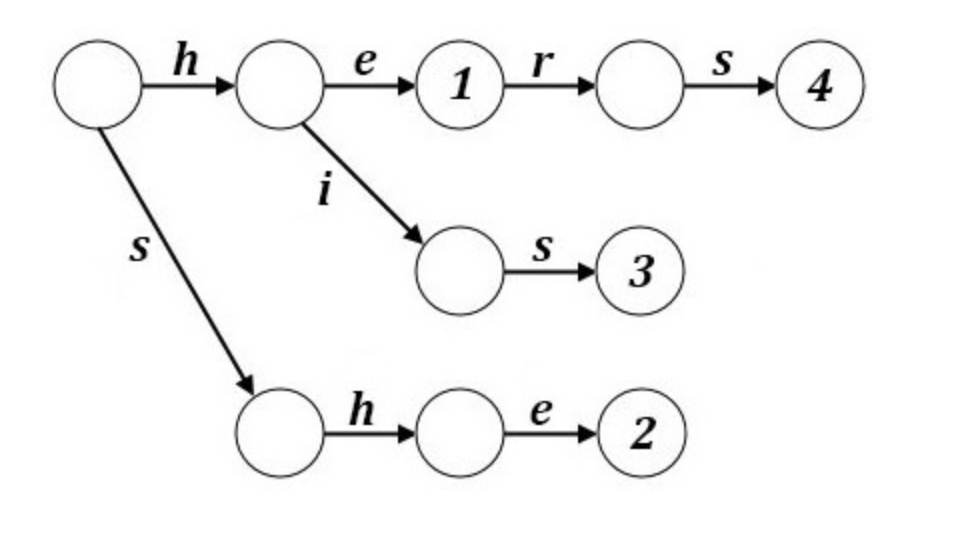
\includegraphics[width=0.6\textwidth]{images/chapter9/trie.png}
                    \label{fig:images/chapter9/trie.png}
        \end{figure}

    \subsection{Задача о словаре}
        Задача о словаре также решается с помощью алгоритма Ахо-Корасик. В этом случае набор образцов представляет собой словарь, а текст проверяется на наличие слов из этого словаря.
        Примером такой задачи может быть проверка текста на наличие запрещенных слов или поиск ключевых слов в большом объеме данных.

    \subsection{Алгоритм Ахо-Корасик}
        \begin{enumerate}[label=\textbf{\arabic* Шаг}:]
            \item \bolditalic{Построение бора}\\
            Строим бор из строк.\\
            Построение выполняется за время $O(m)$, где $m$ — суммарная длина строк.
            \item \bolditalic{Преобразование бора}\\
            
            Обозначим за $[u]$ слово, приводящее в вершину $u$ в боре.\\
            Узлы бора можно понимать как состояния автомата, а корень как начальное состояние.\\
            Узлы бора, в которых заканчиваются строки, становятся терминальными.\\
            Для переходов по автомату заведём в узлах несколько функций:
            
            \begin{itemize}
              \item $parent(u)$ --- возвращает родителя вершины $u$;
              \item $\pi(u) = \delta(\pi(parent(u)), c)$ --- \textbf{суффиксная ссылка}, и существует переход из $parent(u)$ в $u$ по символу $c$;
              \item $\delta(u,c) = \begin{cases}
                  v, & \text{if $v$ is son by symbol $c$ in trie;} \\
                  \text{root}, & \text{if $u$ is root and $u$ has no child by symbol $c$ in trie; $-$ функция перехода}\\
                  \delta(\pi(u), c), & \text{else.}
                \end{cases}$
            \end{itemize}
            
            Мы можем понимать рёбра бора как переходы в автомате по соответствующей букве. Однако одними только рёбрами бора нельзя ограничиваться. Если мы пытаемся выполнить переход по какой-либо букве, а соответствующего ребра в боре нет, то мы тем не менее должны перейти в какое-то состояние. Для этого нам и нужны суффиксные ссылки.\\ 
            Суффиксная ссылка $\pi(u) = v$, если $[v]$ --- максимальный суффикс $[u]$, $[v] \neq [u]$. Функции перехода и суффиксные ссылки можно найти либо алгоритмом обхода в глубину с ленивыми вычислениями, либо с помощью алгоритма обхода в ширину.\\
            
            Из определений выше можно заметить два следующих факта:
            
            \begin{itemize}
              \item функция перехода определена через суффиксную ссылку, а суффиксная ссылка --- через функцию переходов;
              \item для построения суффиксных ссылок необходимо знать информацию только выше по бору от текущей вершины до корня.
            \end{itemize}
            
            Это позволяет реализовать функции поиска переходов по символу и суффиксных ссылок ленивым образом при помощи взаимной рекурсии.

            \begin{figure}[H]
                    \centering
                    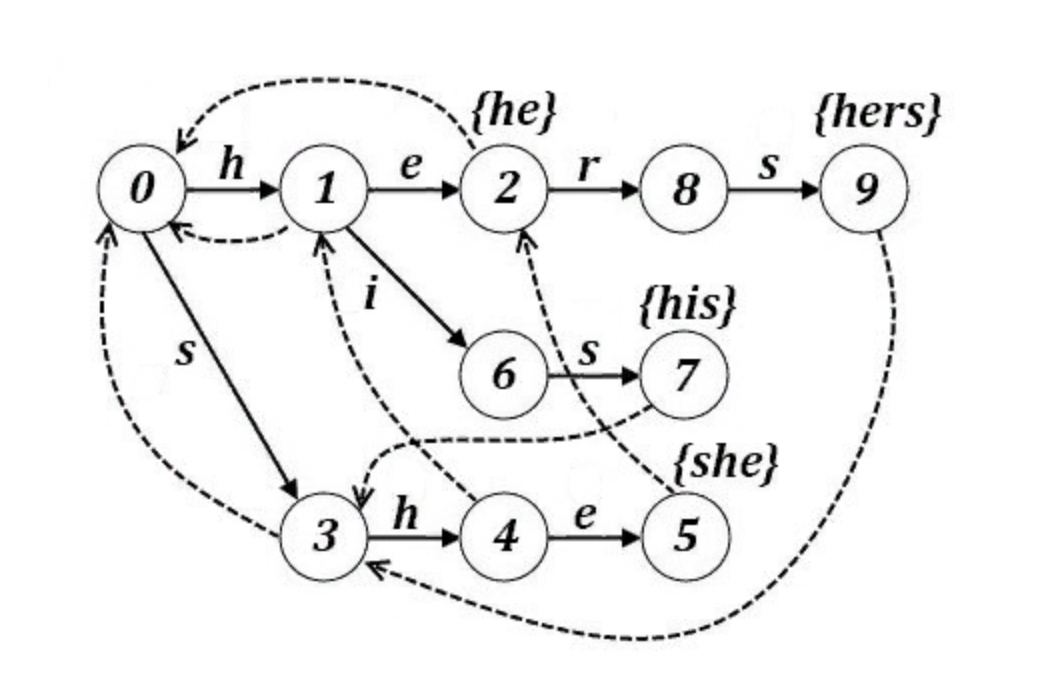
\includegraphics[width=0.6\textwidth]{images/chapter9/acho-korasik-automat-example.png}
                    \label{fig:images/chapter9/acho-korasik-automat-example.png}
                    \caption{Пример автомата Ахо-Корасик}
            \end{figure}

            
            Суффиксные ссылки обозначены пунктиром. Из вершин, для которых они не показаны, суффиксные ссылки ведут в корень.\\
            
            Суффиксная ссылка для каждой вершины $u$ --- это вершина, в которой оканчивается наидлиннейший собственный суффикс строки, соответствующей вершине $u$. Единственный особый случай --- корень бора: для удобства суффиксную ссылку из него проведем в себя же. Например, для вершины 5 с соответствующей ей строкой \textbf{"she"} максимальным подходящим суффиксом является строка \textbf{"he"}. Видим, что такая строка заканчивается в вершине 2. Следовательно, суффиксной ссылкой для вершины 5 является вершина 2.

        
            \item \bolditalic{Построение сжатых суффиксных ссылок}\\
            
            При построении автомата может возникнуть такая ситуация, что ветвление есть не на каждом символе. Тогда можно маленький бамбук заменить одним ребром. Для этого и используются сжатые суффиксные ссылки.
            
            \[
            up(u)=
            \begin{cases}
            \pi(u), & \text{если } \pi(u) \text{ --- терминальная вершина}, \\
            \varnothing, & \text{если } \pi(u) \text{ --- корень}, \\
            up(\pi(u)), & \text{иначе}.
            \end{cases}
            \]
            
            Где $up(u)$ --- сжатая суффиксная ссылка, т.е. ближайшее допускающее состояние (терминал) перехода по суффиксным ссылкам. Аналогично обычным суффиксным ссылкам, сжатые суффиксные ссылки могут быть найдены при помощи ленивой рекурсии.


        \end{enumerate}

\newpage
\section{Сложность алгоритмов}
    Source:
    \begin{enumerate}
        \item Дискретная матемитика и информатика - С.В. Рыбин (2021 г.) $-$ Глава 3.5.8
        \item $\ast$ \href{https://vk.cc/aw2KxE}{Оригинал шпаргалки в высоком разрешении}
    \end{enumerate}
    
    \subsection{Виды сложности}
        Существует несколько видов сложности алгоритмов, которые обычно используются для анализа и оценки эффективности алгоритмов. Некоторые из наиболее распространенных видов сложности включают:
        \begin{enumerate}
            \item \bolditalic{Временная сложность (Time Complexity):}\\
                Это мера количества времени, необходимого для выполнения алгоритма в зависимости от размера входных данных. Оценка временной сложности позволяет предсказать, как будет изменяться время выполнения алгоритма при увеличении размера входных данных. Обычно время работы алгоритма выражается в терминах "O-нотации" (Big O notation), которая описывает его асимптотическое поведение при стремлении размера входных данных к бесконечности. Примеры временной сложности включают $O(1)$ (константная сложность), $O(n)$ (линейная сложность), $O(n^2)$ (квадратичная сложность) и т. д.

            \item \bolditalic{Пространственная сложность (Space Complexity):}\\
                Пространственная сложность алгоритма определяет, сколько дополнительной памяти требуется для выполнения алгоритма в зависимости от размера входных данных. Она измеряется в терминах объема памяти, необходимого для хранения структур данных и временных переменных во время выполнения алгоритма. Пространственная сложность также может быть выражена в O-нотации, аналогично временной сложности.
            \item \bolditalic{Вычислительная сложность (Computational Complexity):}\\
                Вычислительная сложность алгоритма определяет количество вычислительных ресурсов, таких как операции с плавающей точкой, умножения, сравнения и другие, необходимых для выполнения алгоритма. Эта сложность связана с конкретной аппаратной платформой и может варьироваться в зависимости от реализации алгоритма.
            \item \bolditalic{Сложность по другим параметрам:}\\
                В зависимости от конкретной задачи или алгоритма могут быть определены и другие виды сложности, специфичные для этой задачи. Например, в некоторых случаях может быть важной оценка энергетической сложности алгоритма или сложности связи/коммуникации при параллельном выполнении.
        \end{enumerate}
    \subsection{Понятие вычислительной сложности в зависимости от размера входа}
    \begin{itemize}
        \item \bolditalic{Константный} $-$ $T(n)$ $=$ $O(1)$\\
            Любой алгортм, всегда требующий независимо от размера данных одного и того же времени, имеет константную сложность.\\
            Если не считать эффективность в наилучшем случае, в этот класс попадает небольшое число алгоритмов.
        \item \bolditalic{Логарифмический} $-$ $T(n)$ $=$ $O(\log(n))$\\
            Эффективность алгоритма логарифмическая. Алгоритм начинает работать намного медленее с увеличением размера выходных данных ($n$).\\
            Такое время работы характерно для алгоритмов, в которых большая задача делится на маленькие, каждая из которых решается по отдельности. 
        \item \bolditalic{Линейный} $-$ $T(n)$ $=$ $O(n)$\\
            Эффективность алгоритма меняется линейно в зависимости от размера входных данных (обычно такое наблюдается, когда каждый элемент входных данных требуется обработать линейное число раз).\\
            К этому классу относятся алгоритмы, выполняющие сканирование списка, состоящего из $n$ элементов (Например, алгоритм поиска методом последовательного перебора).
        \item \bolditalic{Линейно-логарифмический} $-$ $T(n)$ $=$ $O(n\log(n))$\\
            Такая эффективность характерна для алгоритмов, которые делят большую проблему на маленькие, а затем, решив их, соединяют их решения.\\
            К этому классу относятся большое количество алгоритмов декомпозиции, таких как алгоритмы сортировки, быстрого преобразования Фурье.

        \item \bolditalic{Квадратичный} $-$ $T(n)$ $=$ $O(n^2)$\\
            Обычно, подобная зависимость характеризует эффективность алгоритма, содержищих два встроенных цикла (Например, ряд операций, выполняемых над матрицами размера $n \times n$).
            
        \item \bolditalic{Кубический} $-$ $T(n)$ $=$ $O(n^3)$\\
            Обычно, подобная зависимость характеризует эффективность алгоритма, содержищих три встроенных цикла.
            
        \item \bolditalic{Экспоненциальный} $-$ $T(n)$ $=$ $O(2^n)$\\
            Данная зависимость типична для алгоритмов, выполняющих обработку всех подмножеств некоторого $n$-элементного множества.\\
            Часто термин "экспоненциальный" применятся в широком смысле и означает очень высокий порядок роста (аргумент Big-O).
        \item \bolditalic{Факториальный $-$ $T(n)$ $=$ $O(n!)$}\\
            Характеризует алгоритмы, выполняющих обработку всех перестановок некотрого $n$-элементного множества.
            
    \end{itemize}

    \begin{figure}[H]
                    \centering
                    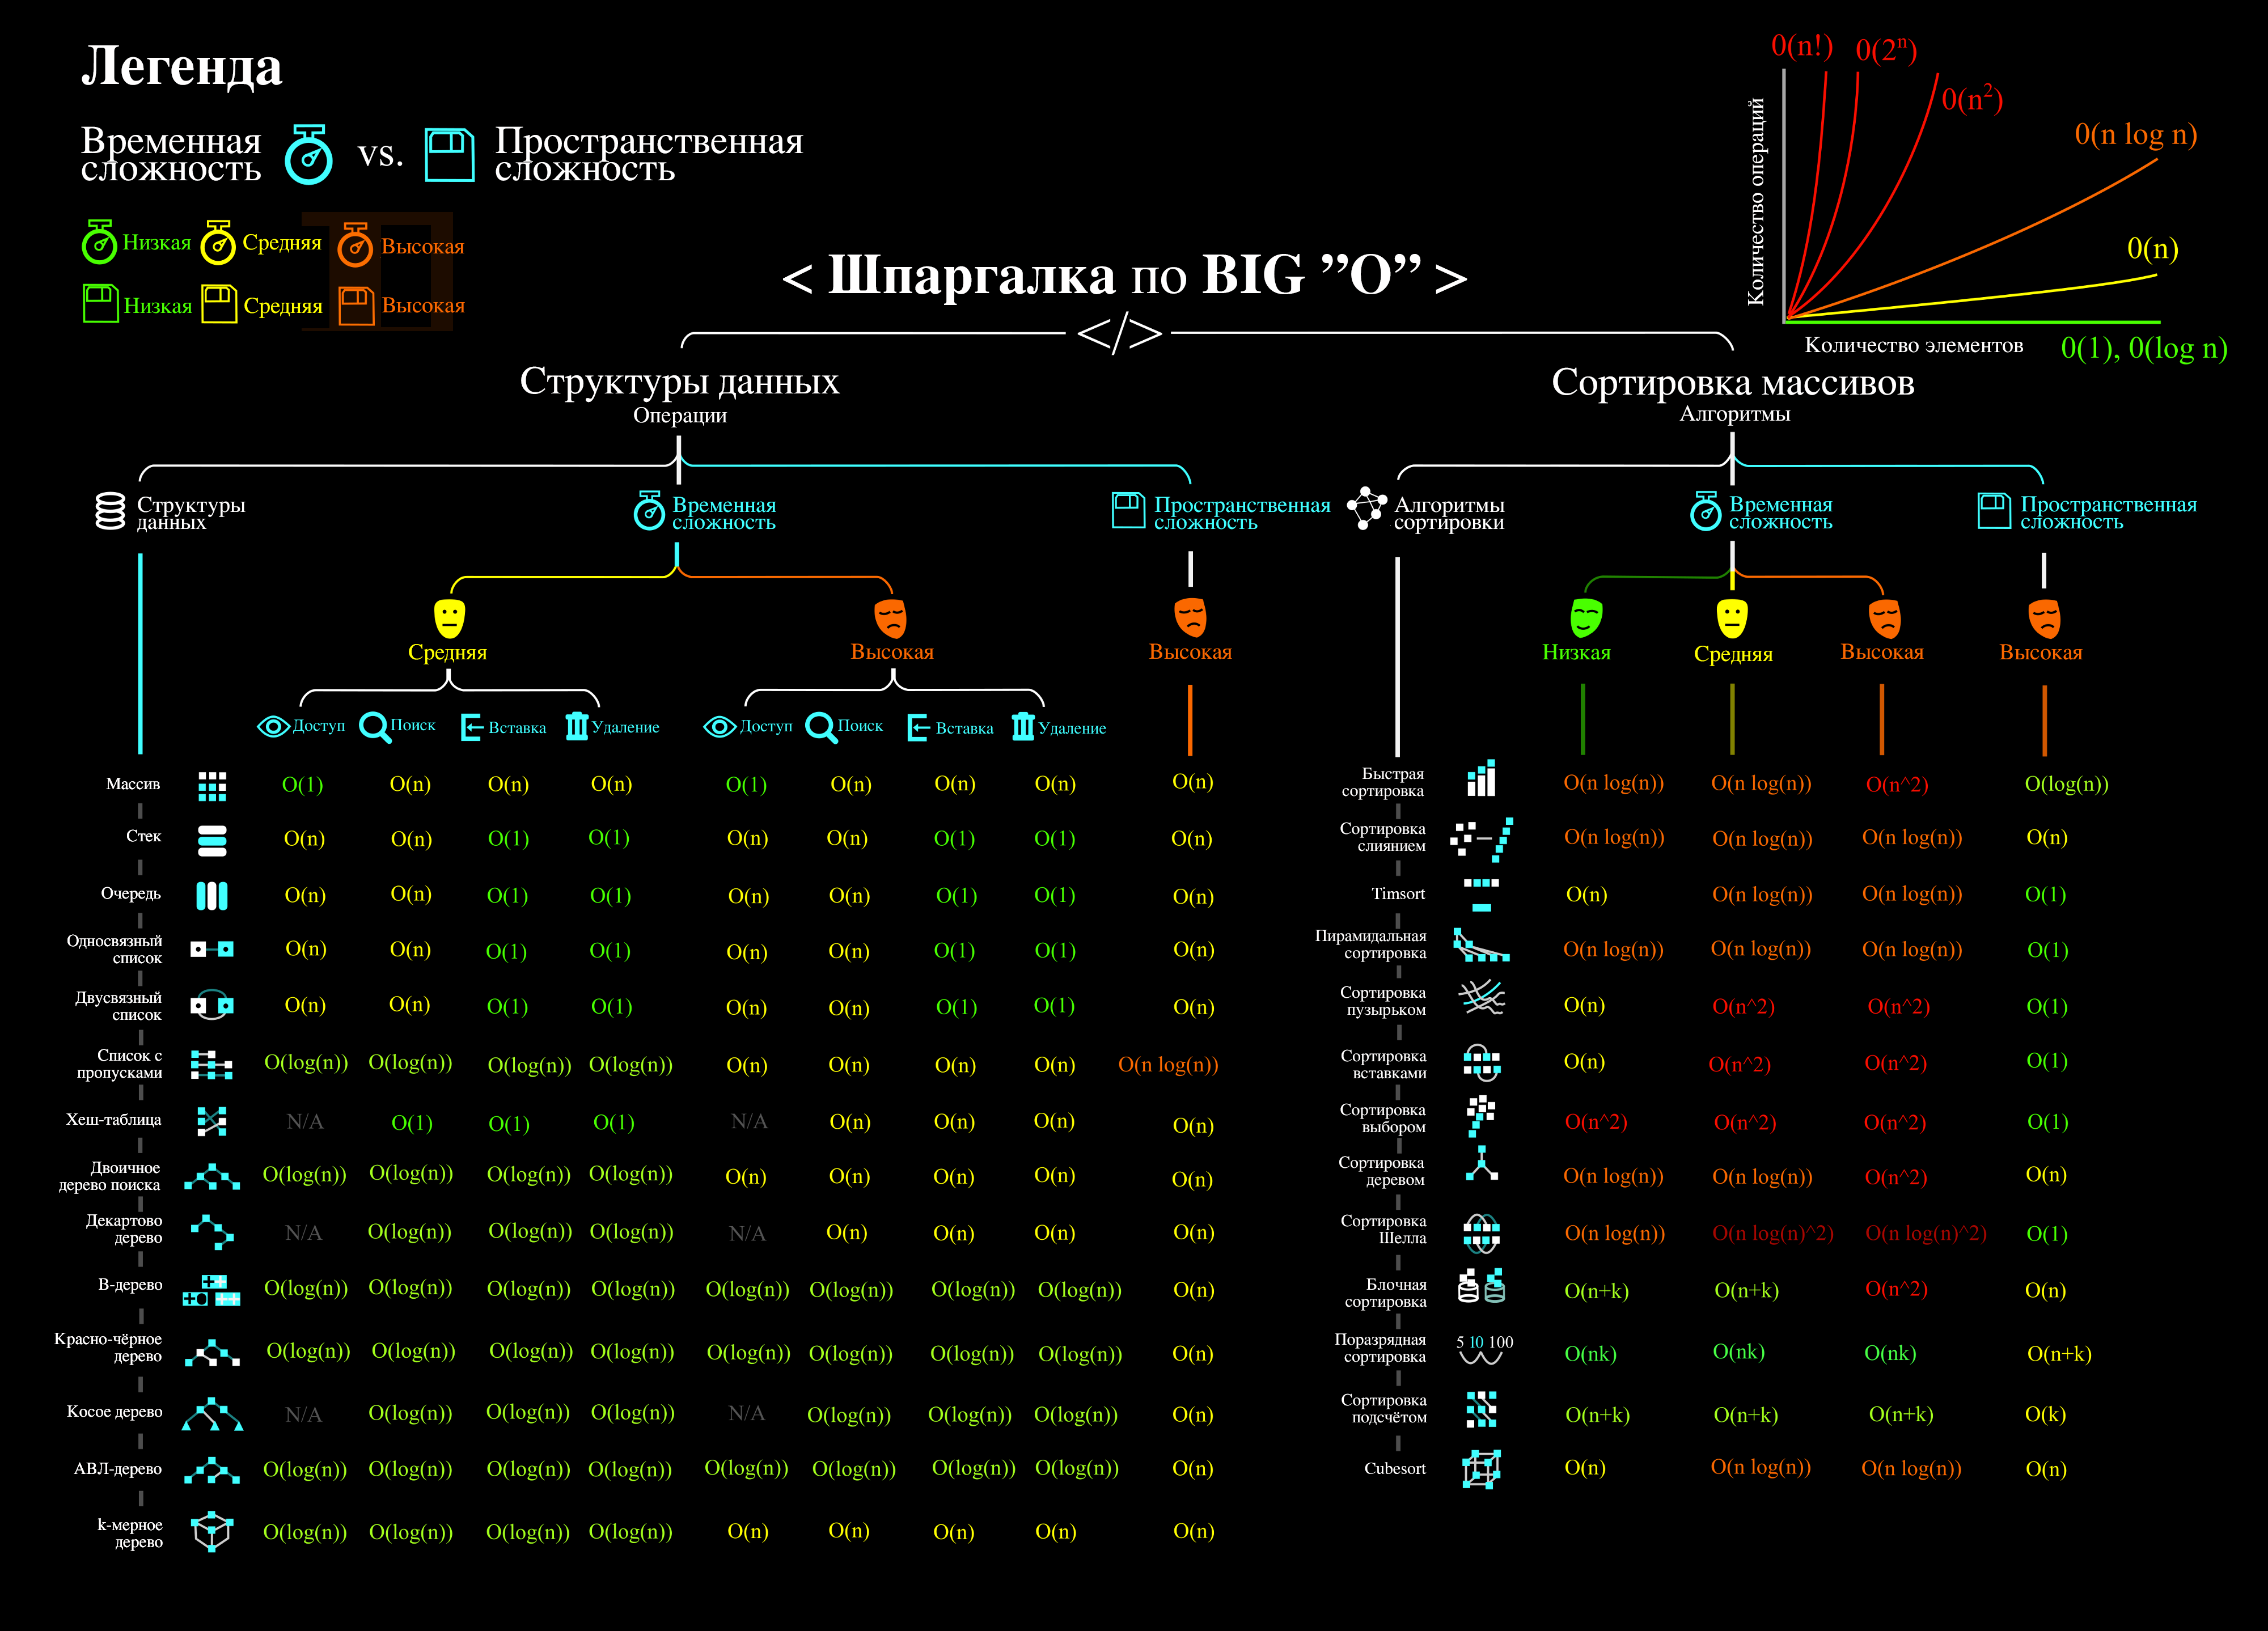
\includegraphics[width=1\textwidth]{images/chapter10/Shpargalka.png}
                    \label{fig:images/chapter10/Shpargalka.png}
                    \caption{Полезная шпаргалка по Big-O}
    \end{figure}
    
    \subsection{Константная сложность на примере vector и unordered\_set:}
    $\ast$ Сделал через гпт, поэтому могут быть ошибки\\
    
    \textbf{std::vector} - это последовательный контейнер, реализованный как динамический массив.\\

    \textbf{std::unordered\_set} - это ассоциативный контейнер, реализованный в виде хэш-таблицы.
    
        \subsubsection{Амортизированная}
            Использование термина "амортизированная константная сложность" означает, что в среднем время выполнения операции является константным, но иногда может быть немного больше, но все равно ограничено.\\

            В случае с \textbf{std::vector}, вставка нового элемента в конец вектора выполняется за \textbf{амортизированное время O(1)}. Это связано с тем, что вектор имеет динамическую структуру данных, которая увеличивает свою внутреннюю емкость при необходимости. Когда вектор заполняется, он выделяет новый блок памяти большего размера и копирует все существующие элементы в новую область. Этот процесс, известный как "реаллокация", происходит реже по мере роста вектора, и поэтому в среднем сложность вставки в конец вектора является амортизированной константой.\\
            
            В\textbf{ std::unordered\_set}, операции вставки, удаления и поиска также имеют \textbf{амортизированную константную сложность O(1)}. Они основаны на использовании хэш-таблицы, которая разрешает коллизии путем создания цепочек элементов с одинаковыми хэшами. Хотя некоторые операции могут потребовать времени O(n) в худшем случае, в среднем время выполнения операций остается константным.\\
            
            \textbf{Таким образом, как для std::vector, так и для std::unordered\_set, операции вставки новых элементов в среднем выполняются за амортизированную константную сложность O(1)}, что обеспечивает эффективность при работе с этими контейнерами.
        \subsubsection{В среднем}
            \textbf{Для std::vector}, вставка нового элемента в конец вектора в среднем имеет сложность O(1), то есть постоянное время. Однако, если вектор достигает своей текущей емкости и требуется выполнить операцию реаллокации, то сложность вставки становится O(n), где n - количество элементов в векторе. Это связано с необходимостью копирования всех элементов в новую область памяти большего размера. В среднем, при последовательной вставке элементов, время выполнения вставки будет близко к O(1), но среди операций может быть несколько дорогих операций реаллокации, что повышает общую сложность.\\

            \textbf{Для std::unordered\_set}, операции вставки, удаления и поиска имеют среднюю сложность O(1) в амортизированном смысле. В хэш-таблице коллизии разрешаются путем создания цепочек элементов, и в большинстве случаев эти операции выполняются за постоянное время. Однако в худшем случае, когда происходит большое количество коллизий, время выполнения операций может достигать O(n), где n - количество элементов в хэш-таблице.\\

            \textbf{Таким образом}, в среднем время выполнения операций вставки, удаления и поиска элементов в std::unordered\_set и вставки элементов в std::vector является постоянным O(1). Но стоит отметить, что в редких случаях, сложность операций может быть выше, особенно при операциях реаллокации вектора или большом количестве коллизий в хэш-таблице.
\section{Изоморфизм графов}
    Source:
    \begin{enumerate}
        \item Дискретная матемитика и информатика - С.В. Рыбин (2021 г.) $-$ Глава 2.1.15
        \item \href{https://habr.com/ru/articles/491846/}{Проверка изоморфности двух графов и поиск изоморфных подграфов: подход на основе анализа NB-Paths | Хабр}
        \item \href{https://habr.com/ru/articles/723328/}{Быстрый поиск изоморфных подграфов | Хабр}
    \end{enumerate}
    \subsection{Задача изоморфизма:}
        \subsubsection{Точный изоморфизм}
            \begin{definition}
                Графы $G_1 = (V_1, E_1)$, $G_2 = (V_2, E_2)$ называются \bolditalic{изоморфными}, если между ними существует взаимо однозначное отображение $\phi$ : $G_1 \longrightarrow G_2$ ($V_1 \longrightarrow V_2$, $E_1 \longrightarrow E_2$), которое сохраняет соответствие между ребрами графов, т.е. для любого ребра $e = (v, u)$ верно:
                \begin{center}
                    $e'$ $=$ $\phi(e)$ $=$ $(\phi(v), \phi(u))$, \quad $(e \in E_1, e' \in E_2)$
                \end{center}
            \end{definition}

            \begin{figure}[H]
                    \centering
                    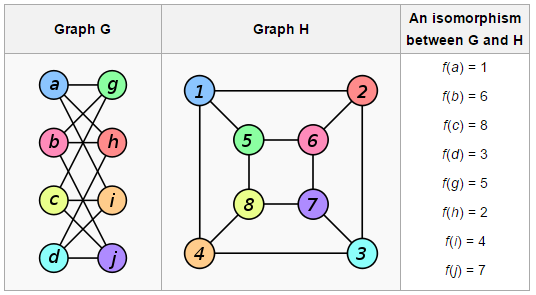
\includegraphics[width=0.7\textwidth]{images/chapter11/isomorphism.png}
                    \label{fig:images/chapter11/isomorphism.png}
                    \caption{Пример изоморфных графов}
            \end{figure}
            
            \textbf{Задача:}\\
            Проверить, являются ли графы $G_1$ и $G_2$ изомофрными.\\
            
            Другими словами, проблема подграфового изоморфизма состоит в определении, являются ли два заданных графа изоморфными, то есть можно ли переставить вершины одного графа так, чтобы получить другой граф.
            
        \subsubsection{Поиск подграфа в графе}
            Пусть у нас определено два графа: большой и малый. Нам требуется найти все такие подграфы большого графа, что они будут изоморфны малому. Большой граф будем называть дата-графом, малый - паттерном

            \begin{figure}[H]
                    \centering
                    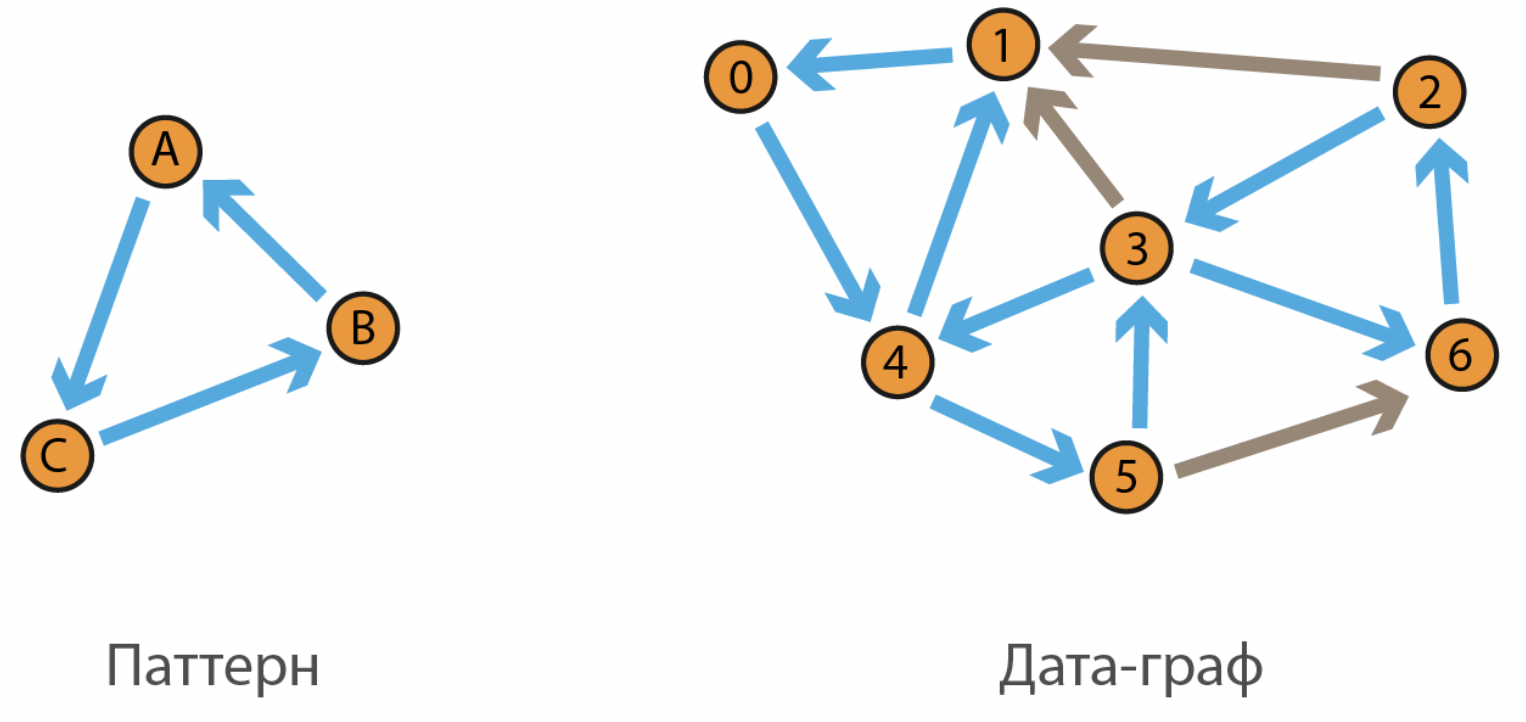
\includegraphics[width=0.7\textwidth]{images/chapter11/subgraph-1.png}
                    \label{fig:images/chapter11/subgraph-1.png}
            \end{figure}

            На рисунке слева изображён паттерн ABC, справа - дата-граф 0123456.\\

            В дата-графе паттерну изоморфны три подграфа:
            \begin{figure}[H]
                    \centering
                    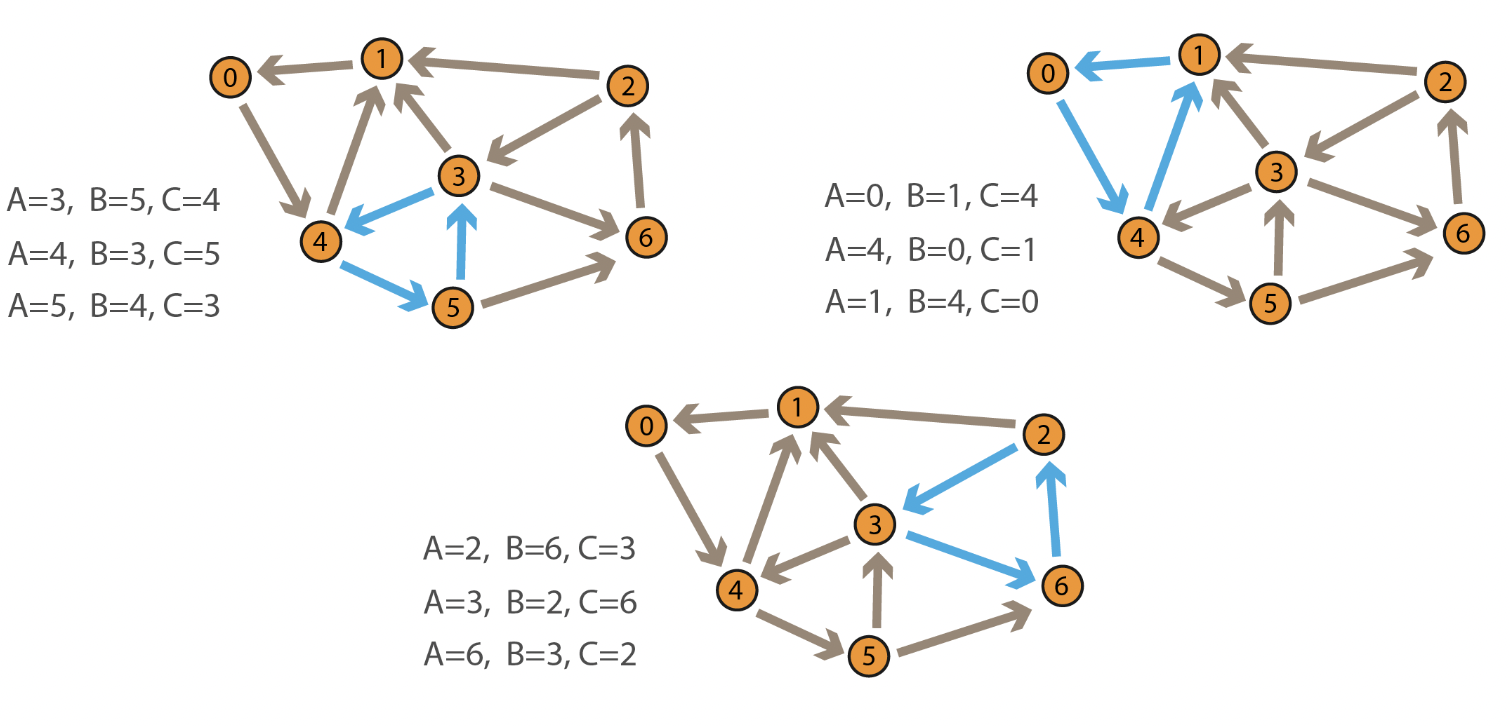
\includegraphics[width=0.9\textwidth]{images/chapter11/subgraph-2.png}
                    \label{fig:images/chapter11/subgraph-2.png}
            \end{figure}
            При этом каждый подграф связан тремя разными комбинациями точек. Такое число комбинаций обусловлено тем, что паттерн симметричен. Если бы в нём совсем не было симметрии, то на каждый подграф приходилась бы ровно одна комбинация. Будем называть такие комбинации изоморфными.\\

            Чтобы найти все изоморфные подграфы перебором, нужно перебрать все возрастающие комбинации вершин дата-графа длины, равной количеству вершин паттерна. Затем нужно построить по ним матрицы смежности и проверить их на изоморфность матрице смежности паттерна.
            
    \subsection{Алгоритм Ульмана (переборный с матрицей)}
        Алгоритм Ульмана основан на методе перебора с использованием матрицы соответствия. Он работает в два этапа: предварительная обработка и рекурсивный поиск.

        \begin{enumerate}
            \item \bolditalic{Предварительная обработка:}
                \begin{itemize}
                    \item Создается матрица соответствия размером $N \times M$, где N - количество вершин в первом графе, а M - количество вершин во втором графе. Изначально все ячейки матрицы установлены в значение "false".
                    \item Для каждой пары вершин (u, v), где u - вершина первого графа, v - вершина второго графа, проверяется их изоморфность:
                    \begin{enumerate}[label=$\star$]
                        \item Если вершины u и v имеют одинаковую степень и нет других вершин, которые уже были сопоставлены с u и v, то устанавливается значение "true" в соответствующей ячейке матрицы.
                    \end{enumerate}
                    \item Повторяется предыдущий шаг до тех пор, пока больше нельзя установить новые соответствия.
                \end{itemize}
            \item \bolditalic{Рекурсивный поиск:}
                \begin{itemize}
                    \item Для каждой пары вершин (u, v), где u - вершина первого графа, v - вершина второго графа, для которых значение "true" установлено в матрице соответствия:
                    \begin{enumerate}[label=$\star$]
                        \item Помечаем вершины u и v как сопоставленные.
                        \item Рекурсивно продолжаем поиск со следующей пары вершин.
                        \item Если поиск успешен для всех пар вершин, то графы считаются изоморфными.
                        \item Если поиск неуспешен, отменяем сопоставление вершин u и v и продолжаем с другой парой вершин.
                    \end{enumerate}
                \end{itemize}
        \end{enumerate}

        Алгоритм Ульмана может быть реализован с использованием рекурсии и обратного отслеживания, чтобы определить все возможные изоморфные соответствия между вершинами двух графов.\\

        Важно отметить, что алгоритм Ульмана имеет экспоненциальную сложность в худшем случае, поэтому он может столкнуться с проблемами при работе с большими графами. Однако, на практике он может быть эффективен для небольших графов или при оптимизациях, таких как использование эвристик и проверка дополнительных условий для исключения некоторых неправильных сопоставлений.
    
    \subsection{Применение изоморфизма}
    \begin{enumerate}
        \item \bolditalic{Генетические Алгоритмы}:\\ 
        Для поиска генов в геноме.
        \item \bolditalic{Распознавание образов и компьютерное зрение:}\\
        Изоморфизм графов используется для сопоставления и распознавания образов. Это может включать сравнение и поиск схожих графов или детектирование объектов на изображении с использованием сопоставления графов.
        \item \bolditalic{Социальные сети и рекомендательные системы:}\\
        Анализ изоморфных графов может быть полезным для исследования социальных сетей, выявления общих паттернов и структурных связей между участниками сети. Кроме того, изоморфные графы могут быть использованы для рекомендации контента или товаров на основе схожих интересов и предпочтений.
    \end{enumerate}

\section{Суффиксные деревья}
Source:
\begin{enumerate}
    \item \href{https://neerc.ifmo.ru/wiki/index.php?title=%D0%A1%D0%B6%D0%B0%D1%82%D0%BE%D0%B5_%D1%81%D1%83%D1%84%D1%84%D0%B8%D0%BA%D1%81%D0%BD%D0%BE%D0%B5_%D0%B4%D0%B5%D1%80%D0%B5%D0%B2%D0%BE}{Сжатое суффиксное дерево (ИТМО конспект)}
    \item \href{https://vec.etu.ru/moodle/mod/resource/view.php?id=155087}{Запись лекции "Алгоритм Ахо-Корасика"}
\end{enumerate}

    \begin{definition}  
        \textbf{Суффиксное дерево} (сжатое суффиксное дерево) $T$ для строки $s$ (где $|s|=n$) — дерево с $n$ листьями, обладающее следующими свойствами:
        \begin{itemize}
            \item Каждая внутренняя вершина дерева имеет не меньше двух детей.
            \item Каждое ребро помечено непустой подстрокой строки $s$.
            \item Никакие два ребра, выходящие из одной вершины, не могут иметь пометок, начинающихся с одного и того же символа.
            \item Дерево должно содержать все суффиксы строки $s$, причем каждый суффикс заканчивается точно в листе и нигде кроме него.
        \end{itemize}
    \end{definition}

    
\textbf{Данное определение порождает следующую проблему:}\\

Рассмотрим дерево для строки $xabxa$: суффикс $xa$ является префиксом суффикса $xabxa$, а, значит, этот суффикс не заканчивается в листе. Для решения проблемы в конце строки $s$ добавляют символ, не входящий в исходный алфавит: \textbf{защитный} символ. Обозначим его как $\$$ (защитный символ). Любой суффикс строки с защитным символом действительно заканчивается в листе и только в листе, т.к. в такой строке не существует двух различных подстрок одинаковой длины, заканчивающихся на $\$$.\\

Далее $n$ — длина строки $s$ с защитным символом.

\begin{figure}[H]
        \centering
        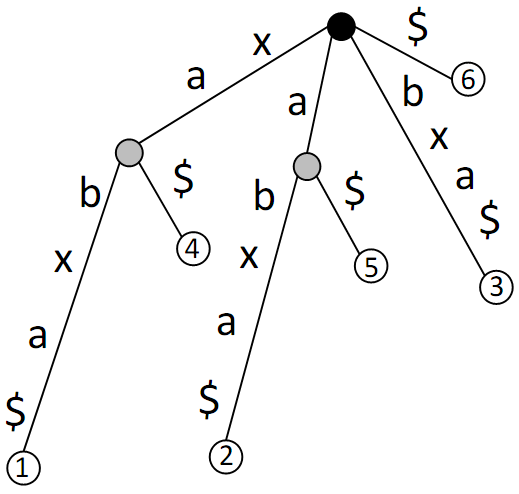
\includegraphics[width=0.3\textwidth]{images/chapter12/Suffix_tree_3.png}
        \label{fig:images/chapter12/Suffix_tree_3.png}
        \caption{Суффиксное дерево для строки $xabxa$
 с защитным символом}
\end{figure}

\textbf{Алгоритм построения суффиксного дерева:}\\
Основная идея алгоритма построения суффиксного дерева состоит в том, чтобы последовательно добавлять суффиксы строки в дерево. Построение дерева выполняется в линейном времени относительно размера входной строки.\\

\begin{enumerate}
    \item Создание корневого узла дерева.

    \item Для каждого суффикса строки:
        \begin{itemize}
            \item Начиная от корневого узла, просматриваем существующие пути по символам суффикса.
            \item Если путь совпадает с текущим символом суффикса, переходим по пути и движемся к следующему символу суффикса.
            \item Если путь не совпадает с текущим символом суффикса, создаем новую ветвь от текущего узла, представляющую оставшийся суффикс.
            \item Если ветвь уже существует, разделяем ее на две части и добавляем новый узел для вставки оставшегося суффикса.
            \item Повторяем процесс для каждого суффикса.
        \end{itemize}
    \item Построение дерева завершается, когда все суффиксы добавлены.
\end{enumerate}

\end{document}